% 10 pages, excluding references
% Abstract 05/12
% Paper 12/12
% CCGrid will be following a double-blind review process
% IEEE two-column conference proceedings template

\documentclass[conference,10pt]{IEEEtran}

\def\BibTeX{{\rm B\kern-.05em{\sc i\kern-.025em b}\kern-.08em
    T\kern-.1667em\lower.7ex\hbox{E}\kern-.125emX}}

\usepackage[utf8]{inputenc}
\usepackage{amsmath, amssymb, amsfonts, colortbl, xspace, todonotes, paralist, multirow, hyperref, pgfplots}
\pgfplotsset{compat=newest}
\hypersetup{
   colorlinks=false,
   pdfborder={0 0 0},
}
\usepackage[english]{babel}
\usepackage{graphicx, color, amssymb, url, xcolor, tikz, pgf, float, subcaption, algorithm,  tabularx}
\usepackage[noend]{algpseudocode}
\usetikzlibrary{trees, shapes, calc, external, fit, arrows, decorations, decorations.pathreplacing, patterns, automata, positioning, arrows.meta, intersections, calligraphy}

% Custom commands
\algnewcommand\algorithmicforeach{\textbf{for each}}
\algdef{S}[FOR]{ForEach}[1]{\algorithmicforeach\ #1\ \algorithmicdo}
\renewcommand{\algorithmicrequire}{\textbf{Input:}}
\renewcommand{\algorithmicensure}{\textbf{Output:}}
\newcommand{\Node}[1]{\ensuremath{\mathrm{Node}_{#1}}\xspace}
\newcommand{\flow}[1]{\ensuremath{\mathit{flow}_{#1}}\xspace}
\newcommand{\file}{\ensuremath{\mathit{File}}\xspace}
\newcommand{\storage}{\ensuremath{\mathit{Storage}}\xspace}
\newcommand{\size}{\ensuremath{\mathit{Size}}\xspace}
\newcommand{\memory}{\ensuremath{\mathit{M}}\xspace}
%\newcommand{\memorymap}{\ensuremath{\mathcal{M}_{map}}\xspace}% not used anymore
\newcommand{\duration}{\mathit{Duration}\xspace}
\newcommand{\bandwidth}{\mathit{Bandwidth}\xspace}
\newcommand{\core}{\mathit{Cores}\xspace}
\newcommand{\submissiontime}{\mathit{SubTime}\xspace}
\newcommand{\emptyflow}{\mathit{ReferenceFlow}\xspace}
%\newcommand{\Endtime}{\mathit{EndTime}\xspace}
\newcommand{\walltime}{\mathit{WallTime}\xspace}
\newcommand{\completiontime}{\mathit{CompletionTime}\xspace}
\newcommand{\start}{\mathit{StartTime}\xspace}
\newcommand{\allocatednode}{\ensuremath\mathit{\sigma}\xspace}
\newcommand{\allocatedcores}{\ensuremath\mathit{\gamma}\xspace}

\newcommand{\fileset}{\ensuremath{\mathbb{F}}\xspace}
\newcommand{\jobset}{\ensuremath{\mathbb{J}}\xspace}
\newcommand{\nodeset}{\ensuremath{\mathbb{N}}\xspace}
\newcommand{\evict}{\ensuremath{\mathcal{V}}\xspace}
\newcommand{\nbloads}{\ensuremath{\mathit{\mathit{Loads}}}\xspace}
\newcommand{\live}{\ensuremath{L}\xspace}
\renewcommand{\algorithmicrequire}{\textbf{Input:}}
\renewcommand{\algorithmicensure}{\textbf{Output:}}

\begin{document}

\title{Locality-aware batch scheduling of I/O intensive workloads}

\maketitle


\begin{abstract}
  Clusters make use of workload schedulers such as
  the Slurm Workload Manager to allocate computing jobs onto
  nodes. These schedulers usually aim at a good trade-off between
  increasing resource utilization and user satisfaction (decreasing
  job waiting time). However, these schedulers are typically unaware
  of jobs sharing large input files, which may happen in data
  intensive scenarios. The same input files may be loaded several
  times, leading to a waste of resources.
   
  We study how to design a \textit{data-aware job scheduler} that is
  able to keep large input files on the computing nodes, without
  impacting other memory needs, and can use previously loaded files to
  \textit{limit data transfers in order to reduce the waiting times of
    jobs}.

  We present three schedulers capable of distributing the load between
  the computing nodes as well as re-using an input file already loaded
  in the memory of some node as much as possible.
  
  We perform simulations using real cluster usage traces to compare
  them to classical job schedulers.  The results show that
  keeping data in local memory between successive jobs and using data
  locality information to schedule jobs allows a reduction in job
  waiting time and a drastic decrease in the amount of data transfers.


  %%%% Longer version below:
  %   Clusters and supercomputers make use of workload schedulers such as
  % the Slurm Workload Manager or OAR to allocate computing jobs onto nodes. These schedulers
  % usually aim at a good trade-off between increasing resource
  % utilization and user satisfaction (decreasing job waiting
  % time). However, these schedulers are typically unaware of jobs
  % sharing large input files: in data-intensive scenarios, tens to
  % hundreds of jobs dedicated to the study of the same multi-GB input
  % file may be successively submitted. Running each of these jobs
  % first requires to load the input file, leading to a large data
  % transfer overhead. Users could manually group some of these
  % tasks into larger jobs to reduce data transfers, but this would result in less granular units that are
  % more difficult to schedule by the resource manager, and would
  % thus result in a larger delay as well. We study how to design a \textit{data-aware
  %   job scheduler} that is able to keep large input files on the 
  % computing nodes, provided this does not impact the memory needs of
  % other jobs, and can use previously loaded files to \textit{limit
  %   data transfers in order to reduce the waiting times of jobs}.

  % We present three schedulers capable of distributing the load between
  % the computing nodes as well as being aware of what the memory of each
  % node contains in order to re-use an input file
  % already loaded in the memory of some node as many times as possible.
  
  
  % We report simulations performed using real cluster usage traces. 
  % Our approach is compared to currently used schedulers in batch systems.
  % The results show that keeping data locally, in memory, between successive
  % jobs and using data locality information to schedule jobs allows a
  % reduction in job waiting time and a drastic decrease in the amount of data
  % transfers.

  
\end{abstract}

%~ \todo[inline]{LM: I changed memory into storage: is it correct ? Carl: I changed back, the point is that these large files are kept in memory with heavy random accesses. There are of course cases where local scratch is sufficient for random accesses, but this not the scenario we've been focusing on. Changed it back.}

\begin{IEEEkeywords}
%~ Batch scheduling,
Job input sharing,
%~ Real workload,
Data-aware,
Job scheduling,
High Performance Data Analytics
%~ Job-input-aware
%~ Communication-aware,
%~ Batch systems
\end{IEEEkeywords}

\section{Introduction}\label{sec.introduction}

To meet the ever-increasing demand for scientific computation power,
High-Performance Computing platforms are typically composed of large
numbers of computation nodes. Scientists typically submit their
computation jobs to a scheduler, which decides the ordering and mapping
of the jobs on the platform. This needs to be performed with particular
care of balancing between resource utilization and user satisfaction, so
as to leverage the computation resources as efficiently as possible,
while avoiding adverse pathological cases that could particularly impact
some users rather than others.

Computation jobs however need data input which, more often than not, can
be very large, notably for many subfields of life science with highly
data-dependent workflows. Loading such data input from the storage
nodes may consume a significant part of the job duration. This load
penalty can however be avoided altogether when the data was actually
already used by the previous job running on the computation node, and
thus still immediately available on the node. Taking care of scheduling
jobs that use the same data input one after the other thus allows to
reduce the jobs completion times, leading to better platform usage
efficiency. Unfortunately, classical job schedulers mostly do not take
data input into account, and thus do not benefit from such data reuse ;
jobs most always have to re-load their data input.

In this paper, we propose to model the benefits of re-using data loads
betwen successive jobs, and we introduce new algorithms that add such
data reuse to the scheduling balance. By tracking which data is loaded
on which node for the scheduled jobs, they are able to significantly
reduce data loads, thus improving both resource utilization and user
satisfaction. We evaluated these algorithms thanks to traces of actual
jobs submissions observed on a large cluster platform. This allows to
assess the effectiveness of our heuristics over a variety of realistic
working sets. This revealed that while our heuristics get slightly worse
results over some working set samples (those which exhibit cluster ample
underuse), most working set samples largely benefit from our heuristics,
leading to interesting benefit overall.

We thus present the following contributions in this paper:
\begin{itemize}
	\item We formalize our model of scheduling data-intensive jobs sharing input files on a cluster (Section~\ref{sec.framework}).
	\item We propose three new schedulers focusing on re-using input files while minimizing evictions and avoiding starvation (Section~\ref{sec.schedulers}).
	\item We extract job information from historical logs of a cluster to build workloads that correspond to the needs and behaviors of real users (Section~\ref{sec.working}).
	\item We implement all three heuristics as well as two state-of-the-art schedulers on a simulator and study the performance (mean stretch and amount of time spent waiting for a file to be loaded) obtained on 44 different workloads (Section~\ref{sec.evaluations}).
	Our evaluation demonstrate that our heuristics in most cases surpass the state of the art schedulers.
	We show that workloads that heavily saturate the cluster
                benefits much more from our strategies which give us
                considerable speed-ups \todo[inline]{Do we want improvement instead of speed-up here?}.
\end{itemize}

\section{Related work}\label{sec.related_work}

\subsection{Scheduling jobs on large clusters}

A various number of workloads managers have emerged 
as a way to meet the rising numbers of high performance computing clusters.
Workload managers like Slurm~\cite{SLURM}, OAR~\cite{oar},
TORQUE~\cite{torque}, LoadLeveler~\cite{loadleveler},
Portable Batch System~\cite{pbs}, SunGrid~\cite{sungrid}
or Load Sharing Facility~\cite{lsf} all offer
various scheduling strategies.

The First-Come-First-Served (FCFS) algorithm is the prevalent default
scheduler on most of these solutions~\cite{survey_workload_manager_and_scheduler}.
Moreover, Slurm is used on most of the TOP500 supercomputers and its default strategy is FCFS~\cite{slurm_website_scheduling} as well.
A backfilling strategy is known to increase
the use of supercomputer resources~\cite{maui}~\cite{New_Backfill}. 
The most commonly used backfilling strategy, called conservative 
backfilling~\cite{Characterization_of_Backfilling}~\cite{Introducing-New-Backfill-based} follows
a simple paradigm: "a job can only be backfilled if it does not
delay a job of higher priority".
We can then safely assume that comparing ourselves to FCFS with and without conservative backfilling can 
bring significant insights on what improvements can be achieved on data-intensive workloads.

Other scheduling strategies exist like 
Maui~\cite{Maui_Scheduler}, Gang scheduling~\cite{gang_scheduling}, 
RASA~\cite{rasa} that use the advantages of both Min-min and Max-min algorithms,
RSDC~\cite{rsdc} that divides large jobs in sub jobs for a more refined scheduling,
or PJSC~\cite{pjsc} and PSP+AC~\cite{PSP_AC} that are a priority-based scheduler; 
however these heuristics do not consider the impact
input re-use could have on data-intensive workloads.
We aim at resolving this issue in this paper.
\todo[inline]{Max: Some citations are quite old, is it an issue?}

\subsection{Using distributed file systems to deal with data-intensive workloads}

Distributed file systems are a solution to ease the access to 
shared input files. They facilitate the execution of I/O-intensive batch
jobs by selecting appropriate storage policies.

Batch-Aware Distributed File System~\cite{Explicit_Control_in_a_Batch-Aware_Distributed_File_System},
is designed to orchestrate large, I/O-intensive batch workloads on remote computing clusters.
HDFS~\cite{hdfs} (Hadoop Distributed File System)
incorporates storage-aware scheduling. 
%It is particularly used to store large volumes of data on a large number of systems.
It migrates a computation closer to where the data is
located, rather than moving the data to where the application is
running, in order to reduce communication.
%~ HDFS is mainly a storage system, thus it uses an historic on files locations to serve as a backup. 

These solutions are mainly storage systems that uses a history of files locations to serve as a backup.
\todo[inline]{Elisabeth: I don't understand the previous sentence. Could it be a history of file locations? How does it serve as a backup? Is it because the files have been duplicated and exist in several places? Max: yes they exist in several places. By default, 2 copies of the data are stored. If one of the machine where the data was stored fails, you can still retrieve the data.}
\todo[inline]{Carl: I find this second point far more important. HDFS is treating the storage point as the actual source of the data, while anything loaded on the nodes in our scenario is just ephemeral copies of a shared storage, which itself has significant levels of redundancy. Individual nodes can sometimes fail in an HPC cluster as well, but those result in the loss of a job, not of primary storage. Max: Ok, I re-wrote this section accordingly.}
In our scenario, we copy the data from an already-redundant system (an online database for example)
and store it locally on the node in an ephemeral way.
Thus, in the event of a crash, we do not manage the data which is already redundant, it simply results in an aborted job.
Secondly, the scheduling can cause issues. Weets et al. describe some problems from
MapReduce~\cite{issue_with_hdfs}, the programming model used in HDFS, in detail.
By not using HDFS or any distributed file system, we avoid these problems altogether. 
Lastly, file systems are particularly efficient when the input data used are identical over time.
In our case, between users, the inputs will be largely different, making distributed file systems less efficient.


%~ However, the main idea is not data re-use, but to
%~ facilitate the execution of I/O intensive batch
%~ jobs by selecting appropriate storage policies
%~ in regards to I/O scoping (creating a custom environment for each job
%~ for data that will be used a lot by the job, thus not accessing the main disk too
%~ much) and space allocation.


\subsection{Using schedulers to deal with data-intensive workloads}

Some schedulers tackle the issue of data-intensive workloads.

A solution can be to minimize network contention by allocating nodes to even out node and
switch contention~\cite{minimize_network_contention}. 
In our model, we are not studying the network topology and consider independent nodes.
This is reasonable, since our main concern is the cross-section bandwidth to a shared storage solution.
\todo[inline]{Carl: Motivating why switch topology of less relevance.}
%~ Moreover, this requires a tree-based network topologies, which is different from our model.
%~ Furthermore, we are scheduling further down the topology (i.e nodes and not switches).
\todo[inline]{Carl: I find the two last two sentences a bit confusing. What are we really trying to say here?
Max: I was trying to say that they use the network topology to make a decision and we don't. 
It was just another way to phrase what you wrote so I removed it. Also, their strategy 
is developed for a tree-based network topology, so it might not work on other topology like a ring or a star?
So, we might want to say that our approach is more generic in regards to the network topology?}

Nikolopoulos et al.~\cite{Nikolopoulos2003AdaptiveSU}
are focusing on a better utilization of idling memory together with 
thrashing limitation.
Our focus will be to control data loads in order to limit eviction
and will thus naturally limit thrashing.
\todo[inline]{Elisabeth: control data loads and limit evictions? Max: Ah yes. I corrected it.}

Agrawal et al.~\cite{Scheduling_Shared_Scans_of_Large_Data_Files}
propose to schedule jobs not sharing a file first
and to use a stochastic model of job arrivals for each input file to maximize re-use.
This work is aimed at the Map-Reduce model and allows to predict future jobs arrivals, two prerequisites that we do not consider.

Equipping each node with a scheduler that follows a work
stealing strategy in order to manage both data locality 
and load balancing is also a solution to reduce data transfers~\cite{Optimizing_load_balancing_and_data_locality_with_data_aware_scheduling}.

Selvarani et al. propose an improved activity-based costing scheduler~\cite{Improved_cost_based_algorithm}
% where the scheduler adapt itself to different application types (CPU intensive, needing high memory, large I/O cost), but our focus will be more generic and aim at maximizing data re-use to meet these needs.
where the processing capacity of each resource is evaluated to make the right decision.
Our approach is more focused on maximizing data re-use on a 
set of identical nodes.

%~ An interesting solution proposed in the context
%~ of the Jacobi-Davidson implementation for solving large
%~ eigenproblems~\cite{loadbalance_and_trashing} tackle both load balancing and memory constraint. For the load balancing, they 
%~ estimate the time needed by the fastest processor to perform the required $m$ jobs. Thus they can equilibrate the load
%~ with this information. In our study we could use a similar strategy by estimating the 
%~ processing time of a job, the length of a file transfer, and the amount of file transfers needed.
%~ To deal with memory constraint the strategy applied in the paper is to check if 
%~ nodes are thrashing data. If yes, it will recede execution of jobs on this node.
%~ The main differences are that they are using dynamic jobs. Also, we would like to 
%~ manage eviction and optimize data reuse during the scheduling phase, instead of
%~ receding execution on nodes.
%~ But is specific to the Jacobi-Davidson method

\section{Framework}\label{sec.framework}

We consider the problem of scheduling a set of $N$ independent jobs,
denoted $\jobset = \{J_1, J_2, \ldots, J_N\}$ on a set of $P$ nodes:
$\nodeset = \{\Node{1}, \Node{2}, \ldots, \Node{P}\}$.
%% LM: to be merged later:
Each node $\Node{i}$ is equipped with $m$ cores noted:
$c^i_1,\ldots,c^i_m$ sharing a memory of size $\memory$.

Each job depends on an input file noted $\file(J_i)$, which is
initially stored in the main shared file system.  During the
processing of a job $J_i$ on $\Node{k}$, file $\file(J_i)$ must be in
the memory of $\Node{k}$. If this is not the case before starting
computation of job $J_i$, then file $\file(J_i)$ is loaded into the
memory.  We denote by $\fileset = \{F_1, F_2, \ldots, F_n\}$ the set
of distinct input files, whose size is denoted by $\size(F_i)$. Each
job runs on a single node, but on different numbers of cores.



Each job $J_i$ has the following attributes:
\begin{itemize}
\item Resource requirement: job $J_i$ requests $\core(J_i)$  cores, such that $1 \leq \core(J_i) \leq m$;
\item Input file: $\file(J_i) \in \fileset$;
\item Submission date: $\submissiontime(J_i)$.
\item Requested running time (or walltime): $\walltime(J_i)$: if not
  finished after this duration, job $J_i$ is killed by the scheduler;
\item Actual running time: $\duration(J_i)$ (unknown to  the scheduler).
\end{itemize}

We do not consider the data output of jobs.

Each of the $N$ jobs must be processed on one of the $P$ nodes.  As
stated earlier, the shared file system initially contains all files
in $\fileset$.  Each node is connected to the file system with a link
of limited bandwidth, denoted by $\bandwidth$: transfering a data of
size $S$ from the shared file system to some node's memory takes a
time $S/\bandwidth$.
The limited bandwidth
as well as the large file sizes are the reasons why we aim at
restricting the amount of data movement.

We consider that the memory of a node, denoted by
$\memory$is only used by the jobs' input files, since all other data are
negligible compared with the input files. We assume that jobs are
devoted a fraction of the memory proportional to the number of
requested cores, so that jobs willing to process large input files
must request large number of cores. This way, we make sure that the
memory of a node is large enough to accomodate all input files of running jobs.
A file stored in the memory of a node can be shared by two jobs $J_i$ and $J_j$ only in the following situations:
\begin{enumerate}
	\item $J_i$ and $J_j$ are computed in parallel on the same node.
	\item $J_i$ and $J_j$ are computed on the same node consecutively.
\end{enumerate}
This can hold true if the file data is accessed through I/O (traditional or memory-mapped),
allowing the same page cache memory pages to serve multiple processes from different jobs.
Otherwise we consider that memory operations of jobs scheduled between
$J_i$ and $J_j$ will cause the file to be evicted.

% We now more formally define the allocation of the jobs to the node and
% their schedule.
% We denote by $\storage(\Node{k}, t)$, the set of files loaded on $\Node{k}$
% at time $t$. The constraint on the limited size of the memory can be
% summarized by:
% $$
% \forall k,\forall t \quad \sum_{F_i\in \storage(\Node{k},t)}
% \size(F_i)\leq \memory.
% $$

For each job $J_i$, the scheduler is in charge of deciding which node
will process $J_i$, and more precisely which cores of this node
allocated to the job, as well as a starting time $t_k$ for $J_i$. Job
$J_i$ is thus allocated a time window from $t_k$ to
$t_k+\walltime(J_i)$ devoted to (i) possibly loading the input file
$\file(J_i)$ in the memory (if it is not already present at time
$t_k$) and (ii) executing job $J(i)$. If the job has not completed at
time $t_k+\walltime(J_i)$, it is killed by the scheduler to ensure
that later jobs are not delayed.  The scheduler must also make sure
that no two jobs are executed simultaneously on the same cores.

It is important to note that the file transfer is done before the computation and cannot be overlapped.
Jobs are non-preemptible: when started, a job is executed through its completion.

Our objective is to obtain an efficient usage of the platform. Each
user submitting jobs is interested in obtaining the result of his jobs
as soon as possible. Hence we focus on the time spent in the system
for each job, also called the flow time (or flow) of the job:
$$
\mathit{Flow}(J_i) = \completiontime(J_i) - \start(J_i).
$$
In the following, we will consider aggregated performance metrics on
job flows, such as average flow or maximum flow. However, the duration
of a job significantly impacts its flow time, and jobs will the same
flow but very different durations do not experience the same quality
of service. To avoid this, the \emph{stretch} metric has been
introduced that compares the actual flow of a job to the one it would
experience on an empty cluster:
\begin{eqnarray*}
\emptyflow(J_i) &=& \duration(J_i) + \frac{\size(\file(J_i))}{\bandwidth}\\
\mathit{stretch}(J_i) &=& \frac{\mathit{Flow}(J_i)}{\emptyflow(J_i)}.
\end{eqnarray*}
The stretch represents the slow-down of a job due to sharing the
platform with other jobs. Considering the stretch
allows to better aggregate performance from small and large jobs.



\section{Job scheduling with input files}\label{sec.schedulers}
%\todo[inline]{Max: Say that we are online, we have no way to know the number or length of future jobs.}
%\todo[inline]{Max: Say that in our case the backfilling is only inside a node and not between multiple nodes.}


Here, we present various schedulers used to allocate jobs to
computing resources. We start with two reference schedulers (FCFS and EFT)
and then move to proposing three locality-aware job schedulers (named
LEA, LEO and LEM). Each of these five schedulers can be used both
without or with backfilling. For the sake of clarity, we first present
the simpler version, without backfilling, before detailing the modifications needed to including backfilling.

As presented above, the task of the scheduler is to allocate a set of
cores of one node
to each job submitted until now: some jobs may be started right away,
while other jobs may be delayed and scheduled later: resource
reservations are made for these jobs. Jobs are presented to the
scheduler in the form of a global queue, sorted by job submission
time. The policies are online algorithms which are called each time
a task completes (thus making cores available) or upon the submission of
a new job.
%Note that in accordance to our framework, each job is allocated to one or several cores of a single node.

%\todo[inline]{Max: Say that the schedule is re-done each time a core is liberated?
%For example with: "Our scheduling policies are online algorithms
%that are called each time a core become available or upon new job's arrival."}




% Some of these methods uses start or completion time as a way to
% schedule each job (section~\ref{subsec.fcfs_eft}) while another compute 
% a score to choose the best node (section~\ref{subsec.score}) and others
% are opting for a mixed strategy between locality and earliest possible start time
% (sections~\ref{subsec.mixed} and~\ref{subsec.opportunistic}).

\subsection{Two schedulers from the state of the art: FCFS and EFT}\label{subsec.fcfs_eft}

A widely-used job scheduler that is typically considered to be efficient is
First-Come-First-Serve (FCFS), detailed in
Algorithm~\ref{algo.fcfs}. Implementing this scheduler requires to
remember the time of next availability for each core. Then, for each job, we look
for the first time when a sufficient number of cores is available, and we allocate the job to
those cores.


\begin{algorithm}[htbp]%\small
\caption{First-Come-First-Serve (FCFS)}\label{algo.fcfs}
\begin{algorithmic}[1]
	\ForEach{$J_i \in$ the jobs queue} %\Comment{The job's queue is sorted by submission times}
        \ForEach{$\Node{k} \in \nodeset$}
        \State Find smallest time $t_k$ such that $\core(J_i)$ cores are available on \Node{k}\label{fcfs.ln.find}
        % Version with backfilling: \State Find smallest time $t_k$ such that $\core(J_i)$ cores are available until at least time $t_k + \walltime(J_i)$ on cores $c_1, ..., c_{\core(J_i)}$ of $\Node{k}$
        \EndFor
        \State Select \Node{k}  with the smallest $t_k$
        \State Schedule $J_i$ on $\core(J_i)$ cores of \Node{k} that are available starting from $t_k$
        \State Mark these cores busy until time $t_k +\walltime(J_i)$
%		\State Cores $c_1, ..., c_{\core(J_i)}$ of $\Node{k}$ are updated to be available at time $t_k + \walltime(J_i)$
%		\State Cores $c_1, ..., c_m$ of $\Node{k}$ are sorted in increasing order of available time \Comment{With a sorted list of cores, writing line 3 is easier}
	\EndFor
	\end{algorithmic}
\end{algorithm}


FCFS is a standard baseline comparison
for job scheduling. However, it is not aware of the capability of the
system to keep a large data file in the memory of a node between the execution of
two consecutive jobs.

A first step towards a locality-aware scheduler
is to select a node for each job not based on the cores' availability
time, but also using the file availability time, based on the file
transfer time. This is the purpose of the Earliest-Finish-Time (or
EFT) scheduler, described in Algorithm~\ref{algo.eft}: by selecting
the node that can effectively start the job at the earliest time, it
minimizes the job completion time. There are three scenarios for the
time $t'_k$ at which the input file of a job $J_i$ is available on
\Node{k}:
\begin{enumerate}
\item A job started before $J_i$ on \Node{k} uses the same input
  file and it is already in memory, thus $t'_k=t_k$;
\item The input file of $J_i$ is not in memory and
  $t'_k=t_k+\frac{\size(\file(J_i))}{\bandwidth}$;
\item The input file of $J_i$ is partially loaded on \Node{k}: this
  happens when some
  job $J_j$ using the same input file has been scheduled on other cores of
  the same node at time $\start(J_j)<t_k$ but the file transfer has not
  completed at time $t_k$. Then the file will be available at time:
  $t'_k = \start(J_j)+\frac{\size(\file(J_i))}{\bandwidth}.$
\end{enumerate}


% Under our model, a fair baseline would be a scheduler capable
% of reducing file transfers while keeping the First-Come-First-Serve
% principle. This scheduler is Earliest-Finish-Time (or EFT).
% It's an enhanced version of FCFS which chooses to schedule a job
% on the node with the earliest available finish time, thus considering
% the time to load the file, and consequently choosing nodes where a file will
% be re-used. 
% \todo[inline]{Max: Say that EFT with bf consider completion time as well.}
% \todo[inline]{Max: The large comment I added in Algo2 should maybe be in a text before with a smaller comment with a reference to the text?}
		
\begin{algorithm}[htbp]%\small
\caption{Earliest-Finish-Time (EFT)}\label{algo.eft}
\begin{algorithmic}[1]
	\ForEach{$J_i \in$ the jobs queue}
		\ForEach{$\Node{k} \in \nodeset$}
			\State Find smallest time $t_k$ such that $\core(J_i)$ cores are available \Node{k}
			% \State Find smallest time $t_k$ such that $\core(J_i)$ cores are available until at least time $t_k + \walltime(J_i)$ on cores $c_1, ..., c_{\core(J_i)}$ of $\Node{k}$
			\State Find time $t_k' \geq t_k$ at which $\file(J_i)$ is available on $\Node{k}$ %\Comment{There are 3 scenarios. 1: the file is already in memory ($t_k' = t_k$), 2: the file is absent ($t_k' = t_k + \frac{\size(\file(J_i))}{\bandwidth}$), 3: the file is partially loaded by another job $J_i'$ started before time $t_k$ ($t_k' = t_k + \frac{\size(\file(J_i))}{\bandwidth} - \bandwidth \times (t_k - \start(J_i'))$)}
		\EndFor
                \State Select \Node{k}  with the smallest $t'_k$
                \State Schedule $J_i$ on $\core(J_i)$ cores of \Node{k} that are available starting from $t_k$
                \State Mark these cores busy until time $t_k +\walltime(J_i)$
                %\State Schedule $J_i$ on the node with the smallest $t_k'$
%		\State Cores $c_1, ..., c_{\core(J_i)}$ of $\Node{k}$ are updated to be available at time $t_k + \walltime(J_i)$
%		\State Cores $c_1, ..., c_m$ of $\Node{k}$ are sorted in increasing order of available time
	\EndFor
\end{algorithmic}
\end{algorithm}

\subsection{Data-locality-based schedulers}

The previous strategies focus on starting (FCFS) or finishing (EFT) a job
as soon as possible, respectively.  Those are good methods
to avoid node starvation and reduce queue times.  However, they
may lead to loading the same input file on a large number of nodes in
the platform, only to minimize immediate queue times. Time is thus spent
loading the input file multiple times. This can affect the global
performance of the system by delaying subsequent jobs.  We present three
strategies that attempt to take data locality into account in a better way to reduce queuing times in the long run by increasing data reuse.

% When the platform is fully loaded, favoring data reuse helps reducing the number of file
% copies and hence reduces queue time in the long run.

The first proposed algorithm called Locality and Eviction Aware (LEA)
and detailed in Algorithm~\ref{algo.lea} aims at a good balance
between node availability and data locality.  We consider three
quantities to rank nodes:
\begin{itemize}
\item The availability time for computation $t_k$;
\item The time needed to complete loading the input file for the job
  on \Node{k} ($t'_k - t_k$);
\item The time required to reload files that need to be evicted before
  loading the input file; this time is computed using all files in
  memory and considering that a fraction of these files need to be
  evicted, corresponding to the fraction of the memory used by the job.
\end{itemize}

The intuition for the third criterion is that if loading a large file
in memory requires the eviction of many other files, these files will not
be available for later jobs and may have to be reloaded.
In the LEA strategy, we put a strong emphasis on data loading, in order
to really favor data locality. Hence, when computing the score for
each node \Node{k}, we sum the previous three quantities, with a weight
$W$ for the second one (loading time). In our experiments, based on
empirical evaluation, we set this value to $W=500$, incidentally roughly
equivalent to the number of nodes.
Note that the other two quantities usually have very different values,
and the availability time is usually much larger than the time for
reloading evicted data. Hence this last criterion is mostly used as a
tie-break in case of equality of the first two criteria.



\begin{algorithm*}[htb]%\small
\caption{Locality and Eviction Aware (LEA)}\label{algo.lea}
\begin{algorithmic}[1]
	\ForEach{$J_i \in$ the jobs queue}
		\ForEach{$\Node{k} \in \nodeset$}
			\State Find smallest time $t_k$ such that $\core(J_i)$ cores are available
			% \State Find smallest time $t_k$ such that $\core(J_i)$ cores are available until at least time $t_k + \walltime(J_i)$ on cores $c_1, ..., c_{\core(J_i)}$ of $\Node{k}$
			\State Find time $t_k'\geq t_k$ at which $\file(J_i)$ is available on $\Node{k}$
			\State $\mathit{LoadOverhead} \gets t_k' - t_k$ %\Comment{It thus gets the load's duration}
%			\State Let $\mathit{sub\_J}$ be the subset of jobs that ends right before time $t_k$ on $\Node{k}$
                        \State Let $\mathcal{F}$ be the set of files in the memory of node \Node{k} at time $t_k$
			\State $\mathit{EvictionPenalty} \gets (\sum_{F_j\in\mathcal{F}}\size(F_j) \times \size(\file(J_i))/\memory)/\bandwidth$
			\State $score_{\Node{k}} \gets t_k + W \times \mathit{LoadOverhead} + \mathit{EvictionPenalty}$
		\EndFor
                \State Select \Node{k} with the smallest $score_{\Node{k}}$
                \State Schedule $J_i$ on $\core(J_i)$ cores of \Node{k} that are available starting from $t_k$
                \State Mark these cores busy until time $t_k +\walltime(J_i)$
	\EndFor
\end{algorithmic}
\end{algorithm*}

%\subsection{LEO}

The LEA strategy puts a dramatic importance on data loads. Hence, it
is very useful when the platform is fully loaded and we can safely
delay the processing of some job to favor data reuse and avoid
unnecessary loads. However, when the platform is not fully loaded,
delaying jobs can be detrimental, as it can increases the response
time for some jobs, without any benefit for other jobs. Our second proposed strategy,
named Locality and Eviction Opportunistic (LEO) and described in Algorithm~\ref{algo.leo}, tries to adapt based
on the current cluster load: if we find some nodes that can process the job
right away, we select the one that will minimize the completion time
(as in the EFT strategy). Otherwise, we assume that the platform is
fully loaded and we apply the previous LEA strategy, to favor data reuse.


\begin{algorithm*}[htb]%\small
\caption{Locality and Eviction Opportunistic (LEO)}\label{algo.leo}
\begin{algorithmic}[1]
	\ForEach{$J_i \in$ the jobs queue}
		\ForEach{$\Node{k} \in \nodeset$}
			\State Find smallest time $t_k$ such that $\core(J_i)$ cores are available
			% \State Find smallest time $t_k$ such that $\core(J_i)$ cores are available until at least time $t_k + \walltime(J_i)$ on cores $c_1, ..., c_{\core(J_i)}$ of $\Node{k}$
			\State Find time $t_k'\geq t_k$ at which $\file(J_i)$ is available on $\Node{k}$
			\State $\mathit{LoadOverhead} \gets t_k' - t_k$ %\Comment{It thus gets the load's duration}
                        \State Let $\mathcal{F}$ be the set of files in the memory of node \Node{k} at time $t_k$
			\State $\mathit{EvictionPenalty} \gets (\sum_{F_j\in\mathcal{F}}\size(F_j) \times \size(\file(J_i))/\memory)/\bandwidth$
			\If{$t_k = \mathit{current\_time}$}
				\State $score_{\Node{k}} \gets t'_k$
			\Else
			         \State $score_{\Node{k}} \gets t_k + W \times \mathit{LoadOverhead} + \mathit{EvictionPenalty}$
			\EndIf
		\EndFor
                \State Select \Node{k} with the smallest $score_{\Node{k}}$
                \State Schedule $J_i$ on $\core(J_i)$ cores of \Node{k} that are available starting from $t_k$
                \State Mark these cores busy until time $t_k +\walltime(J_i)$
	\EndFor
\end{algorithmic}
\end{algorithm*}

We present a third strategy called Locality and Eviction Mixed (LEM)
and described in Algorithm~\ref{algo.lem} that takes a similar approach to
LEO but performs a simple mix between the EFT and the LEA strategies:
when the load of the platform (measured as the number of nodes running
at least one job) is above a criterion, the LEA strategy is applied,
otherwise the EFT strategy is used.
 

\begin{algorithm}[htb]%\small
\caption{Locality and Eviction Mixed (LEM)}\label{algo.lem}
\begin{algorithmic}[1]
	\ForEach{$J_i \in$ the jobs queue}
		\State $\mathit{load} \gets$  percentage of nodes running at least one job at current time
		\If{$\mathit{load} < 80$}
			\State $EFT(\jobset,\nodeset)$
		\Else
			\State $LEA(\jobset,\nodeset)$
		\EndIf
	\EndFor
\end{algorithmic}
\end{algorithm}



\subsection{Adding backfilling to all strategies}

As mentioned above, backfilling has been proposed to increase the
performance of job schedulers, by allowing jobs with lower priority to be
scheduled before jobs with higher priority. In our setting, the
priority is directly linked to the submission order: if $J_i$ is
submitted before $J_j$, then $J_i$ has a higher priority than $J_j$.
\todo[inline]{Sam: it seems to me we don't really want to talk about
"priority", but rather submission order?\\LM: I prefer to keep the
``priority'' name, as it is the classical term used when presenting
backfilling, but I tried to link it to submission order, ok?}
In order to avoid jobs
being perpetually delayed, bounds have to be set on how already-scheduled
jobs can be affected by backfilling. As discussed above,
Conservative Backfilling is the most restrictive version and one of
the most commonly-used strategies to improve cluster utilization. It
forbids any modification on the resource
reservations of high-priority jobs: a job may be scheduled
before other jobs that appear earlier in the queue, provided that it
does not impact the starting time of these jobs.


For each of the previous scheduling strategies, we consider a variant
using conservative backfilling (suffixed by -BF).  To add
backfilling, Algorithms~\ref{algo.fcfs}, \ref{algo.eft},
\ref{algo.lea} and~\ref{algo.leo} have to be modified: we change the
choice of the earliest time when resources are available for a job
(Line~\ref{fcfs.ln.find}). Instead of considering the time at which
cores are (indefinitely) available, we look for an availability time
window starting at $t_k$ long enough to hold the
job. Specifically, we change Line~\ref{fcfs.ln.find} into:
\begin{algorithmic}[0]
  \State $\ref{fcfs.ln.find}'$: Find smallest time $t_k$ such that $\core(J_i)$ cores are
  available from $t_k$ until $t_k + \walltime(J_i)$ on $\Node{k}$
\end{algorithmic}

Note that this requires the algorithm to store  the whole occupation profile of
each core (with availability and unavailability times), whereas the
version of each scheduler without backfilling simply requires the time
of last job completion.


\begin{figure}[t]
\pgfplotsset{every tick label/.append style={font=\large}}
\definecolor{color1}{HTML}{CEDEF0}
\definecolor{color2}{HTML}{9D9AD9}
\definecolor{color3}{HTML}{6B9BD1}
\centering\scalebox{0.75}{
\begin{tikzpicture}\begin{axis}
[ font=\footnotesize,
  ytick style={draw=none},
  xtick style={draw=none},
  unit vector ratio*=1 1 1,
  axis lines = middle,
  enlarge x limits = {value=.1,upper},
  enlarge y limits = {value=.05,upper},
  ylabel={\large Cores},
  xlabel={\large Time},
  ylabel near ticks,
  xlabel near ticks,
  const plot,
  stack plots=false,
  area style,
  ytick={1,...,3},
  yticklabels={},  
  xtick={1,...,5},
  extra y ticks={0,1,2},
  extra x ticks={0,1,2,3,4,5},
  extra y tick style={yticklabel={$C_{\pgfmathprintnumber{\tick}}$}}] 
\addplot[fill=color1] coordinates {(0,0) (0,1) (1,1) (1,0)} node at (current path bounding box.center) {\large Job 1}; 
\addplot[fill=color2] coordinates {(1,0) (1,2) (2,2) (2,0)} node at (current path bounding box.center) {\large Job 2}; 
\addplot[fill=color3] coordinates {(2,0) (2,1) (3,1) (3,0)} node at (current path bounding box.center) {\large Job 3};
\addplot[fill=color3,opacity=0.7] coordinates {(0,1) (0,2) (1,2) (1,1)} node at (current path bounding box.center) {\large Job 3};
\node (A) at (2, 1) {};
\node (B) at (1, 1.5) {};
\draw [->,-{Latex[round]},line width=1.5] (A) edge (B);
\end{axis}\end{tikzpicture}}
\caption{Example of the benefit of conservative backfilling. Job 3 was submitted after job 2 but can be backfilled to start earlier without delaying the start time of job 2.}
\end{figure}

\todo[inline]{Max: Do we want to say:
"On a node, when choosing the cores that will be used for a job among the available ones, 
we choose the ones with the lowest index.
This allow to optimize the cores utilization and reduces the risk of
covering available cores that will need backfilling to be used.
Additionally, when backfilling a job, the cores with the smallest next 
start time of a job are chosen, in order to fill as much as possible
the nodes."\\
LM: I don't think we need to mention this. Tie-breaking using smallest
index is the default behavior in most systems.}

\section{Working with information from a real workload and cluster\todo[inline]{Max: Another name for this section?}}\label{sec.working}


Actual workloads at HPC resources shared by a great number of users with diverse needs can contain structures
that are non-trivial to replicate in a fully artificial simulated job pattern. We believe that this is especially
true for data-dependent patterns, where a project might launch a burst of jobs using the same file just a few thousand
core hours in length, then be quiet for a long time processing the results, and then launch another such burst.
However, changing the scheduling strategy of a production cluster for
scheduling research would disrupt the community using this cluster.


For this reason, we choose to perform simulations based on logs of
historically submitted jobs, containing their exact submission time,
size, stated walltime, and actual duration\footnote{Links to the logs
  are omitted for double-blind review but will be made
  available in the final submission.}.  
Since explicit data dependencies are not encoded in SLURM job
specifications, we do not have access to the actual input files of
these jobs. We thus create an artificial data dependency pattern that
replicates user behaviors.
We consider two jobs $J_i$ and $J_j$. These jobs are considered to
share their input file if they match the three following requirements:
\begin{enumerate}
	\item $\core(J_i) = \core(J_j)$, i.e., they are requesting the same number of cores.
	\item $J_i$ and $J_j$ were submitted by the same user.
	\item $J_i$ and $J_j$ were submitted within an 800 seconds
          time frame. We consider this timeframe to be a reasonable amount of time for a user to submit all of their jobs using the same input file.
\end{enumerate}
Otherwise, we consider that $J_i$ and $J_j$ are using distinct input files.


The platform where the logs have been extracted
consist of 486 nodes with 20 cores each, with most of them
having 128GB of RAM, and a few 256GB and 1024GB nodes.

Having three different node sizes does not fit the proposed model and
raises new challenges: some input files are too large to be processed
on a subset of nodes. However, a small input file may be processed on
both nodes with small and large memory.
Thus, in addition to the scheduling problem, a load balancing problem arises.
%For example, should a job using a file of size $M_1$ be scheduled on a node of size $M_2$?
Indeed, the scheduler needs to be able to manage each subset of nodes as an independent 
resource that needs to avoid starvation while also not being saturated
in case of a sudden batch of jobs requesting a node of its size. This
problem is left for future work as we focus in the present paper on
data locality.
Consequently, we consider here that the platform is made of 486 homogeneous nodes of size 
$\memory = 128GB$.


We consider that these jobs are dedicated to processing their input
file. Hence, the more cores the job requests, 
the larger its input file. This allows to compute the size of files as follows:
$$\size(\file(i)) =\frac{\core(J_i)}{20} \times 128GB$$

The utilization levels in the log of the platform are typically high ($>90\%$), but
not fully consistently so. The vast majority of jobs on these
resources are single-node jobs\todo[inline]{LM: but we consider only
single-node jobs, right?? Max: Yes, I added a sentence to detail what 
we do to multi-nodes jobs. Do we want to keep it like that?}, even sometimes single-core jobs.
The few multi-nodes jobs are replaced by as many single-node jobs as necessary to represent the same occupation.
We notice that job
durations extend up to 10 days, while some jobs only last a few minutes. We do not claim that this is an ideal job submission strategy,
but rather it is an empirical observation of an actual user community including, but not exclusively consisting of, many subfields of the life sciences with highly data-dependent workflows.

Each application scenario evaluated in the next section represents one day's worth of log history from the real workload,
processed in a realistic scheduling environment steady state also determined by the logs.
The way we collect and schedule jobs from the log's history is represented in Figure~\ref{fig.workload}.
\begin{figure*}[tb]
\definecolor{blue}{rgb}{0.38, 0.51, 0.71} %glaucous, 97,130,181, #6182B5
\definecolor{darkblue}{RGB}{17, 42, 60} % 112A3C
\definecolor{red}{RGB}{175, 49, 39} % AF3127
\definecolor{otherred}{RGB}{171,78,78}
\definecolor{orange}{RGB}{237, 126, 75} 
\definecolor{green}{RGB}{104, 174, 89} 
\definecolor{palegreen}{RGB}{197, 184, 104} 
\definecolor{yellow}{RGB}{250, 199, 70} % FAC764
\definecolor{brokenwhite}{RGB}{218, 192, 166} % DAC0A6
\definecolor{brokengrey}{rgb}{0.77, 0.76, 0.82} % {196,194,209}, C4C2D1
\centering\scalebox{1}{
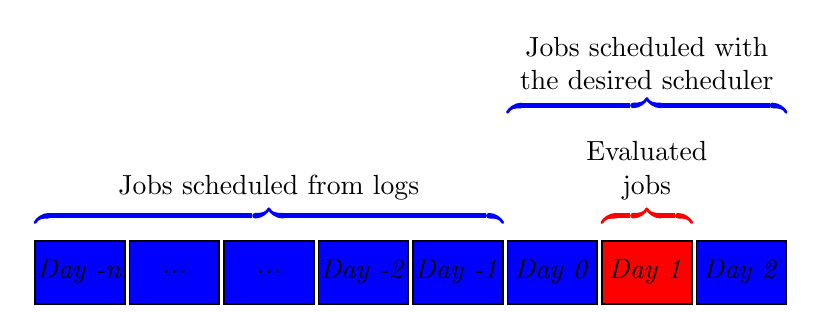
\begin{tikzpicture}[semithick, > = {Stealth[scale=1.25]}, shorten > = 1pt,]
    \def\x{1}\def\y{1}
    \draw[color=black, fill=blue] (1.2*1*\x+0.03, 0.7) rectangle (1.2*2*\x-0.03, -0.1) node[midway] {\textit{Day -n}}; 
    \draw[color=black, fill=blue] (1.2*2*\x+0.03, 0.7) rectangle (1.2*3*\x-0.03, -0.1) node[midway] {\textit{...}}; 
    \draw[color=black, fill=blue] (1.2*3*\x+0.03, 0.7) rectangle (1.2*4*\x-0.03, -0.1) node[midway] {\textit{...}}; 
    \draw[color=black, fill=blue] (1.2*4*\x+0.03, 0.7) rectangle (1.2*5*\x-0.03, -0.1) node[midway] {\textit{Day -2}}; 
    \draw[color=black, fill=blue] (1.2*5*\x+0.03, 0.7) rectangle (1.2*6*\x-0.03, -0.1) node[midway] {\textit{Day -1}}; 
    \draw[color=black, fill=blue] (1.2*6*\x+0.03, 0.7) rectangle (1.2*7*\x-0.03, -0.1) node[midway] {\textit{Day 0}}; 
    \draw[color=black, fill=red] (1.2*7*\x+0.03, 0.7) rectangle (1.2*8*\x-0.03, -0.1) node[midway] {\textit{Day 1}}; 
    \draw[color=black, fill=blue] (1.2*8*\x+0.03, 0.7) rectangle (1.2*9*\x-0.03, -0.1) node[midway] {\textit{Day 2}}; 
    %~ \draw[color=black, fill=blue] (1.2*4*\x+0.03, 0.7) rectangle (1.2*5*\x-0.03, -0.1) node[midway] {Day 3}; 
    %~ \draw[color=black, fill=blue] (1.2*5*\x+0.03, 0.7) rectangle (1.2*6*\x-0.03, -0.1) node[midway] {Day 4}; 
    %~ \draw[color=black, fill=blue] (1.2*6*\x+0.03, 0.7) rectangle (1.2*7*\x-0.03, -0.1) node[midway] {Day 5}; 
    %~ \draw[color=black, fill=blue] (1.2*7*\x+0.03, 0.7) rectangle (1.2*8*\x-0.03, -0.1) node[midway] {Day 6}; 
    %~ \draw[color=black, fill=blue] (1.2*8*\x+0.03, 0.7) rectangle (1.2*9*\x-0.03, -0.1) node[midway] {Day 7}; 
    %~ \draw[color=black, fill=blue] (1.2*9*\x+0.03, 0.7) rectangle (1.2*10*\x-0.03, -0.1) node[midway] {Day 8}; 
    %~ \draw[color=black, fill=blue] (1.2*10*\x+0.03, 0.7) rectangle (1.2*11*\x-0.03, -0.1) node[midway] {Day 9}; 
    %~ \draw[color=black, fill=blue] (1.2*11*\x+0.03, 0.7) rectangle (1.2*12*\x-0.03, -0.1) node[midway] {Day 10}; 
    \draw [pen colour={blue},decorate,line width=2pt,decoration = {calligraphic brace,raise=-2pt,amplitude=5pt}] (1.2*1*\x+0.03, 1) -- node[pos=0.5,above=2pt,black,align=center]{Jobs scheduled from logs} (1.2*6*\x-0.03, 1);
    \draw [pen colour={blue},decorate,line width=2pt,decoration = {calligraphic brace,raise=-2pt,amplitude=5pt}] (1.2*6*\x+0.03, 2.4) -- node[pos=0.5,above=2pt,black,align=center]{Jobs scheduled with\\the desired scheduler} (1.2*9*\x-0.03, 2.4);
    %~ \draw [pen colour={blue},decorate,line width=2pt,decoration = {calligraphic brace,raise=-2pt,amplitude=5pt}] (1.2*4*\x+0.03, 1) -- node[pos=0.5,above=2pt,black,align=center]{Days used to collect all the jobs submitted before \textit{Day 3}} (1.2*12*\x-0.03, 1);
    \draw [pen colour={red},decorate,line width=2pt,decoration = {calligraphic brace,raise=-2pt,amplitude=5pt}] (1.2*7*\x+0.03, 1) -- node[pos=0.5,above=2pt,black,align=center]{Evaluated\\jobs} (1.2*8*\x-0.03, 1);
  \end{tikzpicture}
}
\caption{Methodology followed to schedule and evaluate jobs from a specific day while avoiding edge effects.}\label{fig.workload}
\label{fig.ex}
\end{figure*}
On the real cluster, when a job finishes, all of its metadata
are written to a file corresponding to the day during which the job finished.
%~ This information contains the node that was attributed, the real job's duration, the walltime, 
%~ the number of cores required, the user that submitted the job, the submission time, 
%~ the start and end time.
Our goal is to schedule and evaluate all the jobs submitted on 
\textit{Day 1} with the settings in which they were on the real cluster.
In order to get all the jobs that were submitted on \textit{Day 1}, we
look into the logs of days 0 to 10. Indeed, almost all jobs do not last for more than 10 days,
thus we should be able to cover the vast majority of jobs that were actually submitted on 
\textit{Day 1}.
With this process, we also gather jobs that were started on \textit{Day 0} and \textit{Day 2}. 
Thanks to this, jobs of \textit{Day 1} are respectively preceded and succeeded with jobs from \textit{Day 0}
and \textit{Day 2} in order to place \textit{Day 1} in its "real environment",
i.e., in the situation in which it was on the real cluster while also avoiding any side effect.
Jobs from \textit{Day -1, -2, ..., -n} are jobs that were submitted before \textit{Day 0} and that are still running at the beginning of \textit{Day 0}.
We use the information from the log's history to start these jobs on the nodes
where they were actually executed and at the times at which they really started.
This will exactly replicate the state of the cluster just before \textit{Day 0}.
To summarize, before \textit{Day 0}, jobs are placed on the cluster
following the log's history. Starting from \textit{Day 0} we 
use one of our schedulers. We then only evaluate jobs submitted on \textit{Day 1}
to avoid side effects.

\section{Performance evaluation and analysis}\label{sec.evaluations}

Below, we present the results of experimental evaluations conducted 
on 44 days extracted from logs of historical submitted jobs.

\subsection{Settings}

All strategies as well as the two baselines have been implemented on
a simulator that we developed\footnote{\url{https://github.com/user-for-double-blind-submission/Locality-aware-batch-scheduling-of-I-O-intensive-workloads}}.
We compute the flow and stretch for all jobs after their termination.

% For each job, its flow will be computed after its termination.
% The flow of a job is the total amount of time the job spent in the system, i.e.,
% the duration from the submission time to the completion time. The flow
% allows to evaluate both the queue time and the time spent loading its input file.
% We measure the obtained performance with the mean
% stretch from all jobs of \textit{Day 1}.

% The stretch of a job is the flow of the job divided
% by the flow the job would have gotten if it was scheduled on an empty cluster.
% They are denoted respectively $Flow(J_i)$ and $\emptyflow(J_i)$.

% \begin{equation}
% Flow(J_i) = \completiontime(J_i) - \submissiontime(J_i)
% \end{equation}

% \begin{equation}
% \emptyflow(J_i) = \duration(J_i) + \frac{\size(\file(J_i))}{\bandwidth}
% \end{equation}

% The stretch of each job is computed as follows:
% \begin{equation}
% Stretch_{J_i} = \frac{Flow(J_i)}{\emptyflow(J_i)}
% \end{equation}

\todo[inline]{Max: Do we need a table to recap the acronyms and
  strategies or reading the section scheduler is sufficient to know
  the acronyms? LM: no need for such table I guess}
We also evaluate the total amount of time spent waiting for a file to be available.
Our main competitors on these metrics are FCFS and EFT, with and without backfilling.
\todo[inline]{Max: Do we need more in this setting section?}
Let's first study the behavior of our schedulers on different workloads,
offering different saturations of the cluster.

\subsection{An underutilized cluster, LEA issues and the appeal of LEM}\label{sec.07-16}

\subsubsection{Results\todo[inline]{Max: Maybe use paragraphs instead of subsubsection?}}

\begin{figure}[t]\centering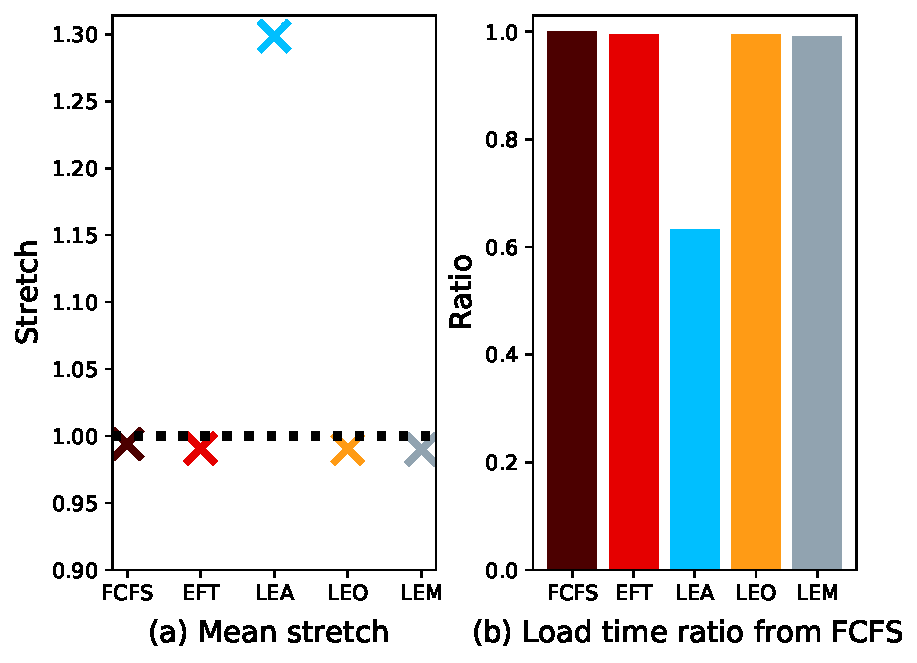
\includegraphics[width=1\linewidth]{../MBSS/plot/Results_FCFS_Score_Backfill_2022-07-16->2022-07-16_V10000_Mean_Stretch_Total_waiting_for_a_load_time_and_transfer_time_450_128_32_256_4_1024.pdf}\caption{Average stretch of all jobs evaluated and total transfer time on July 16.}\label{stretch.07-16}\end{figure}
%~ \begin{figure}[t]\centering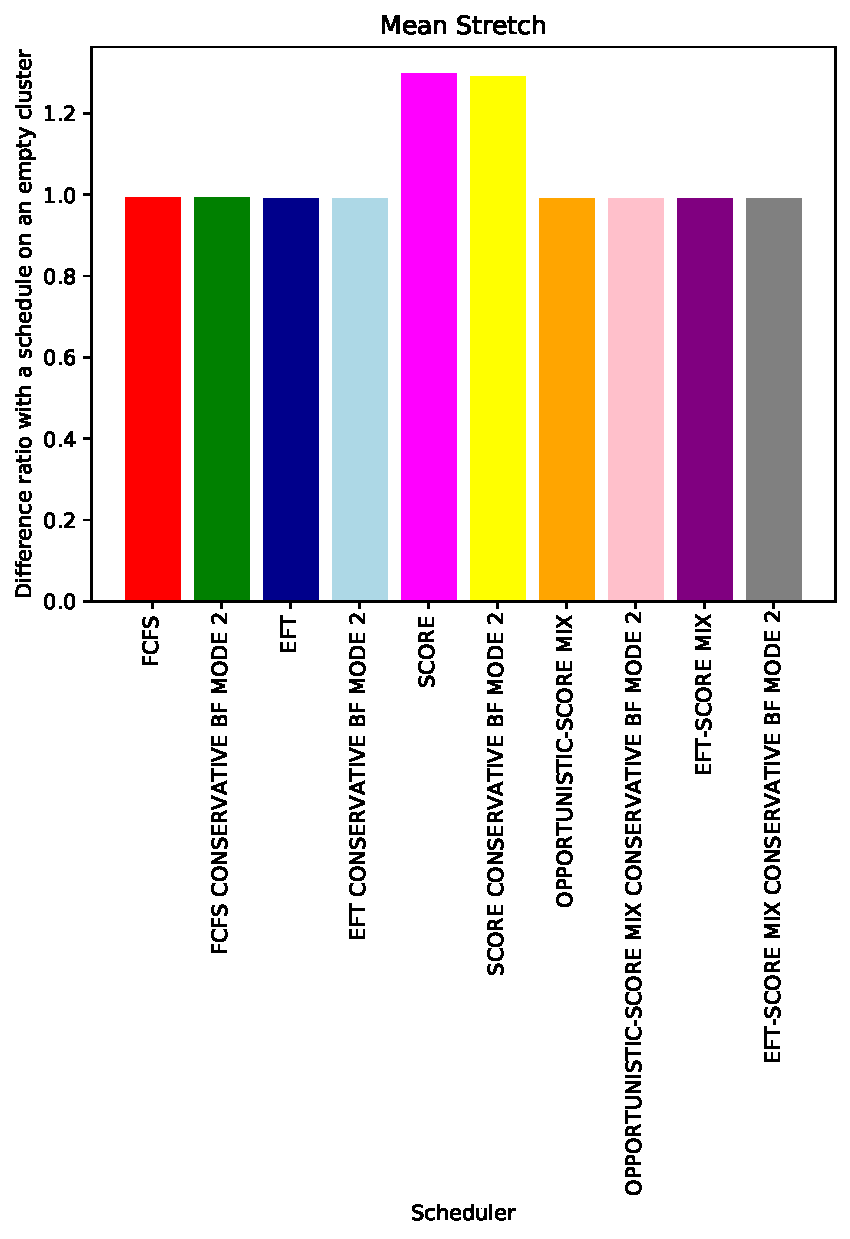
\includegraphics[width=1\linewidth]{../MBSS/plot/Results_FCFS_Score_Backfill_2022-07-16->2022-07-16_V10000_Mean_Stretch_450_128_32_256_4_1024.pdf}\caption{Average stretch of all jobs evaluated on July 16.}\label{stretch.07-16}\end{figure}
%~ \begin{figure}[t]\centering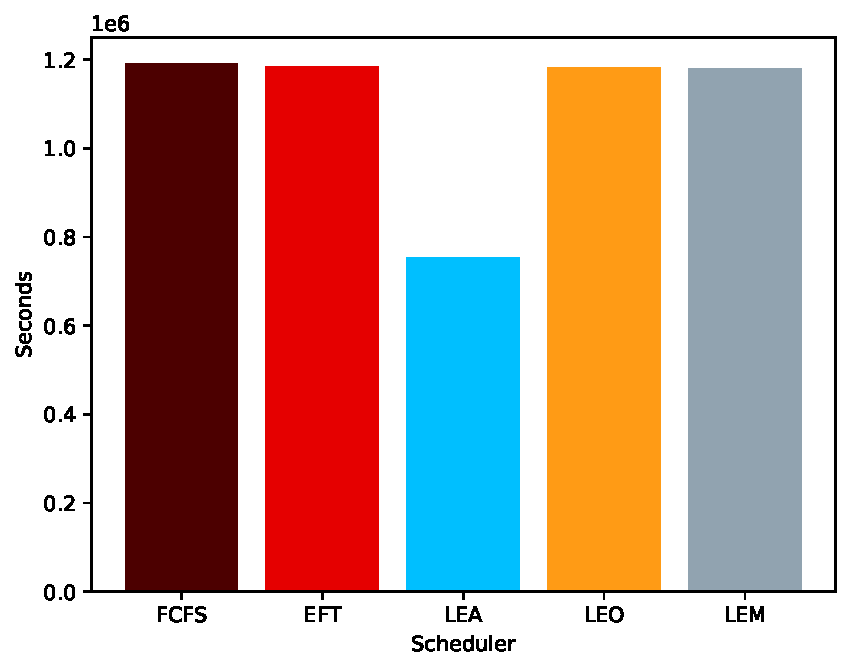
\includegraphics[width=1\linewidth]{../MBSS/plot/Results_FCFS_Score_Backfill_2022-07-16->2022-07-16_V10000_Total_waiting_for_a_load_time_and_transfer_time_450_128_32_256_4_1024.pdf}\caption{Amount of time spent waiting for a file to be available on July 16.}\label{load.07-16}\end{figure}
\begin{figure}[t]\centering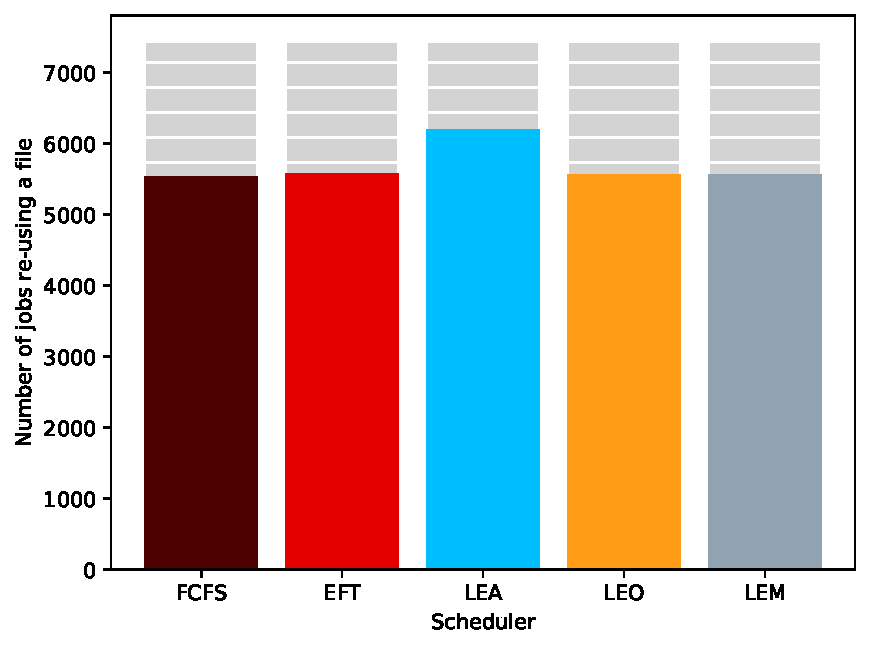
\includegraphics[width=1\linewidth]{../MBSS/plot/Results_FCFS_Score_Backfill_2022-07-16->2022-07-16_V10000_Number_of_data_reuse_450_128_32_256_4_1024.pdf}\caption{Number of evaluated jobs re-using a data on July 16.}\label{reuse.07-16}\end{figure}

Figure~\ref{stretch.07-16}a shows us, for each scheduler, the mean stretch from all jobs
submitted on July 16.
\todo[inline]{Should we say on July 16 or on July 16?
Carl: I prefer July
16. A comment is also that file names containing > might cause
production problems if the conference accepts tex files for
submission. Max: Okay I've putted July 16. I'll remove the arrows once we have our final figures.}
The horizontal black dotted line corresponds to a stretch of 1.
This stretch is obtained if all jobs 
are scheduled on an empty cluster. It corresponds to the waiting time of each job being exactly
the time it takes to load the input file.
FCFS, EFT, LEO and LEM have mean stretches close to 1.
EFT, LEO and LEM have a slight benefit over FCFS thanks to file re-use.
LEA is 23\% slower.

Figures~\ref{stretch.07-16}b and \ref{reuse.07-16} 
both gives us similar information. The first one
shows the total amount of time spent 
waiting for a file to be ready before starting the computation,
relative to the total waiting time of FCFS.
The second figure
shows the number of jobs that re-used a file,
i.e,. the file was already in memory or 
another job was already loading the file.
The gray background denote the total
number of jobs.
On both of these figures, LEA is the outlier:
it re-uses input files for more jobs and consequently the total time spent waiting for a load is lower.

\subsubsection{Understanding LEA's poor performance}

\begin{figure}[t]\centering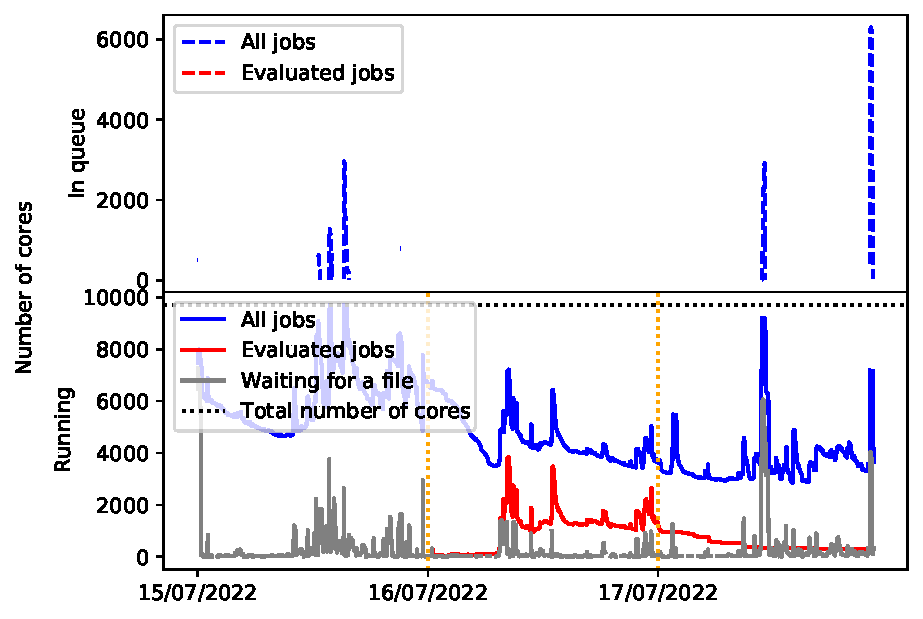
\includegraphics[width=1\linewidth]{../MBSS/plot/Cluster_usage/2022-07-16->2022-07-16_V10000_Fcfs_Used_nodes_Reduced_450_128_32_256_4_1024_core_by_core.pdf}\caption{Visualization of the utilization rate of the cluster on the workload of July 16 with FCFS.}\label{07_16_cluster_usage_fcfs}\end{figure}
\begin{figure}[t]\centering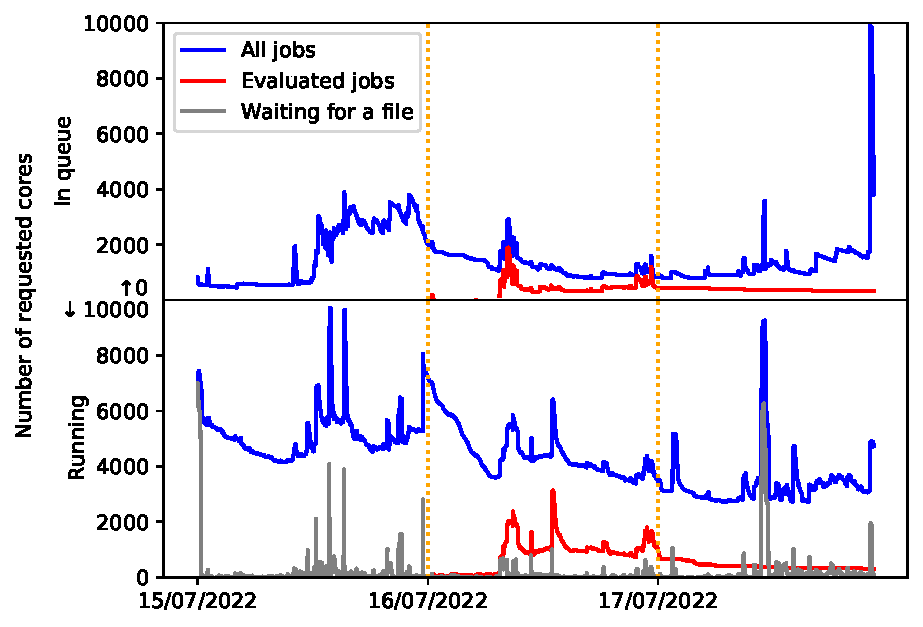
\includegraphics[width=1\linewidth]{../MBSS/plot/Cluster_usage/2022-07-16->2022-07-16_V10000_Fcfs_with_a_score_x500_x1_x0_x0_Used_nodes_Reduced_450_128_32_256_4_1024_core_by_core.pdf}\caption{Visualization of the utilization rate of the cluster on the workload of July 16 with LEA.}\label{07_16_cluster_usage_lea}\end{figure}
\begin{figure}[t]\begin{subfigure}[b]{0.49\linewidth}\centering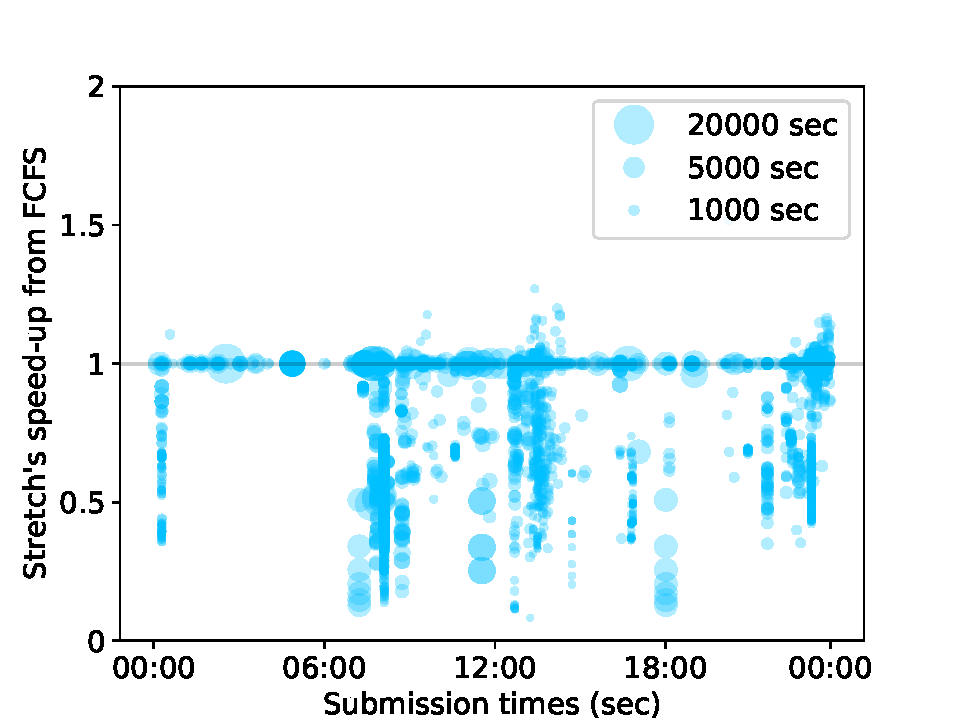
\includegraphics[width=1\linewidth]{../MBSS/plot/Stretch_times/Stretch_times_FCFS_LEA_2022-07-16->2022-07-16_V10000_450_128_32_256_4_1024.pdf}\caption{With LEA.}\label{07_16_fcfs_vs_lea}\end{subfigure}
\begin{subfigure}[b]{0.49\linewidth}\centering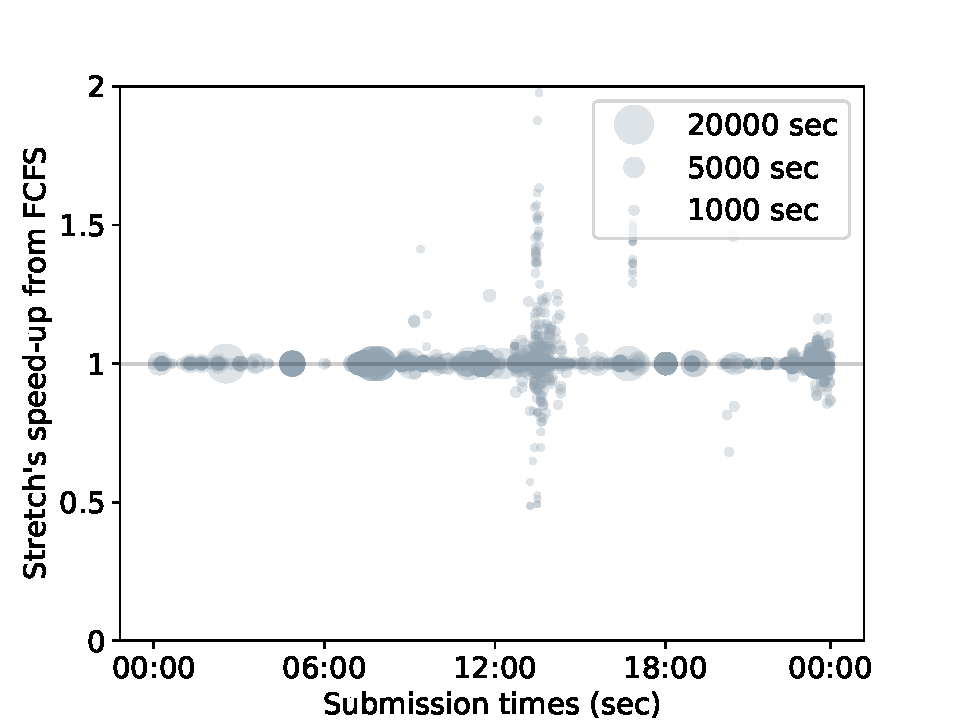
\includegraphics[width=1\linewidth]{../MBSS/plot/Stretch_times/Stretch_times_FCFS_LEM_2022-07-16->2022-07-16_V10000_450_128_32_256_4_1024.pdf}\caption{With LEM.}\label{07_16_fcfs_vs_lem}\end{subfigure}\caption{Stretch times of each job compared to FCFS on the workload of July 16.}\end{figure}

To understand the issues LEA encounters on this workload, we need to study the cluster's usage over time.
Figure~\ref{07_16_cluster_usage_fcfs} shows us a visual representation of 
our cluster's usage when using FCFS.
The Y axis represents the number of requested cores either running on a
node (lower half) or in the queue of jobs waiting to be executed (top
half). The maximum is the total number of cores on our cluster: 9720.
The blue line shows the number of cores from all jobs.
%~ The solid blue line shows the number of cores from all jobs.
%~ The dashed blue line shows the additional number of cores that would be needed
%~ to run all the jobs in the queue at a given time (this would thus be the number
%~ of used cores if all the jobs where running in parallel).
The red lines show the number of cores used by the evaluated jobs, i.e.
those jobs that have their submission time within our evaluation window. Thus, this forms a subset
of the set indicated by the the blue line.
If a line is present in the top half, it means that some jobs could not be scheduled
and are thus waiting in the queue of available jobs. 
A node could have available cores that are still too few to accommodate some jobs.
This explains why jobs can be in the queue, even if the lower half does not reach the maximum.
The gray line represents the number of cores currently loading a file.
Lastly, the orange lines delimits the submission times of our 
evaluated jobs, in other words it's our evaluation window.
\todo[inline]{Tell what dotted orange lines are. Max: Okay done.}

By looking at the top half of Figure~\ref{07_16_cluster_usage_fcfs}
we understand that the job queue is empty most of the time.
In this situation, FCFS is very efficient. The earliest available node is in
most cases a node that can start the job immediately, explaining the mean stretch close to 1 in Figure~\ref{stretch.07-16}a.
LEO is a strategy that uses the earliest available time $t_k$ of a node to decide if it should compute a score like LEA,
that puts a large weight on transfer time\todo[inline]{Max: We use $t_k$ as the "earliest available time to compute x cores on node k" in the schedulers section. Can we use it here?} or weigh equally $t_k$, the transfer and eviction durations. 
Thus, on underused clusters, LEO has a behavior close to EFT, while trying to minimize evictions.
Similarly, LEM switches between EFT and LEA depending on the cluster's usage.
On this particular workload the cluster's usage is under 80\%, so LEM behaves similarly to EFT.
On the contrary, LEA favors data re-use over an early start time for a job.
On an underused cluster it increases starvation.
We can notice this when looking at
Figure~\ref{07_16_cluster_usage_lea}. It shows the cluster usage when using LEA.
We can notice that it uses fewer cores, notably before the first vertical orange dotted line. 
This translates into a larger queue of jobs that you can see on the top half of the figure.
For LEA, most of the jobs in this queue are jobs that already have a valid copy of their file loaded on a node. 
The benefit of scheduling these jobs immediately on another node and loading the file appears
inferior to waiting for a file re-use for LEA and thus creates this queue of jobs that does not exist for FCFS. 
The consequence in terms of stretch is immediately noticeable on Figure~\ref{07_16_fcfs_vs_lea}.
This visualization shows the stretch's speed-up of each job compared to FCFS.
The size of a circle is proportional to the job's duration.
On the workload of July 16, we can observe, below a speed-up of 1, columns of jobs submitted at the same time and
with the same duration (so probably jobs using the same file),
meaning LEA is waiting to re-use the files before starting the jobs,
whereas FCFS paid the cost of loading the file, but started the jobs
earlier than LEA, leading to a 
smaller flow with FCFS.
From Figure~\ref{07_16_fcfs_vs_lem} concerning LEM, we can see that most jobs have a speed-up close to 1, showing 
that LEM does not fall into LEA's pathological case.

To summarize, on an underutilized cluster, LEA's focus on locality
does not allow optimal utilization of the cluster, whereas LEO and LEM, thanks
to their flexibility,
achieve performance identical to EFT.

\subsection{An almost saturated cluster, the weakness of LEM and the resilience of LEO}\label{sec.09-09}

In the previous section, we saw the benefit of using LEO or LEM over LEA.
Here we evaluate our strategies on a workload that almost saturated the
cluster, underlining the weakness of LEM.

\subsubsection{Results}

\begin{figure}[t]\centering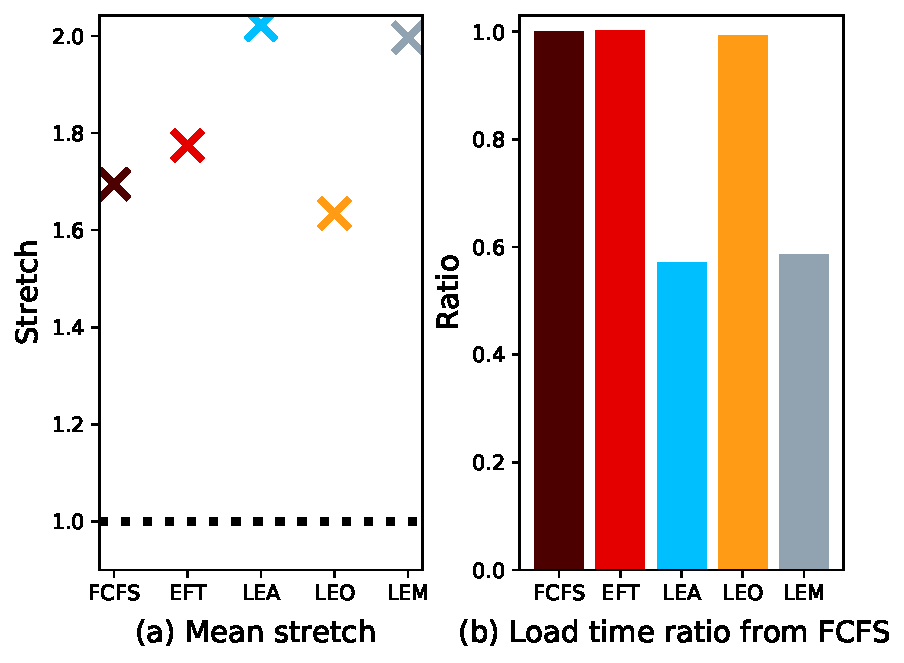
\includegraphics[width=1\linewidth]{../MBSS/plot/Results_FCFS_Score_Backfill_2022-09-09->2022-09-09_V10000_Mean_Stretch_Total_waiting_for_a_load_time_and_transfer_time_450_128_32_256_4_1024.pdf}\caption{Average stretch of all jobs evaluated and total load time on September 09.}\label{stretch.09-09}\end{figure}
%~ \begin{figure}[t]\centering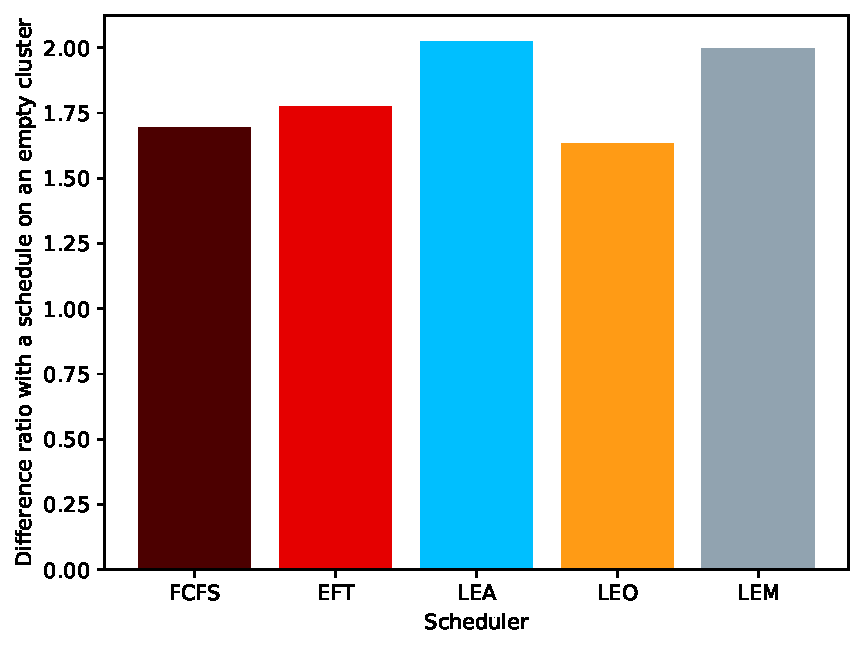
\includegraphics[width=1\linewidth]{../MBSS/plot/Results_FCFS_Score_Backfill_2022-09-09->2022-09-09_V10000_Mean_Stretch_450_128_32_256_4_1024.pdf}\caption{Average stretch of all jobs evaluated on September 09.}
%~ \label{stretch.09-09}\end{figure}
%~ \begin{figure}[t]\centering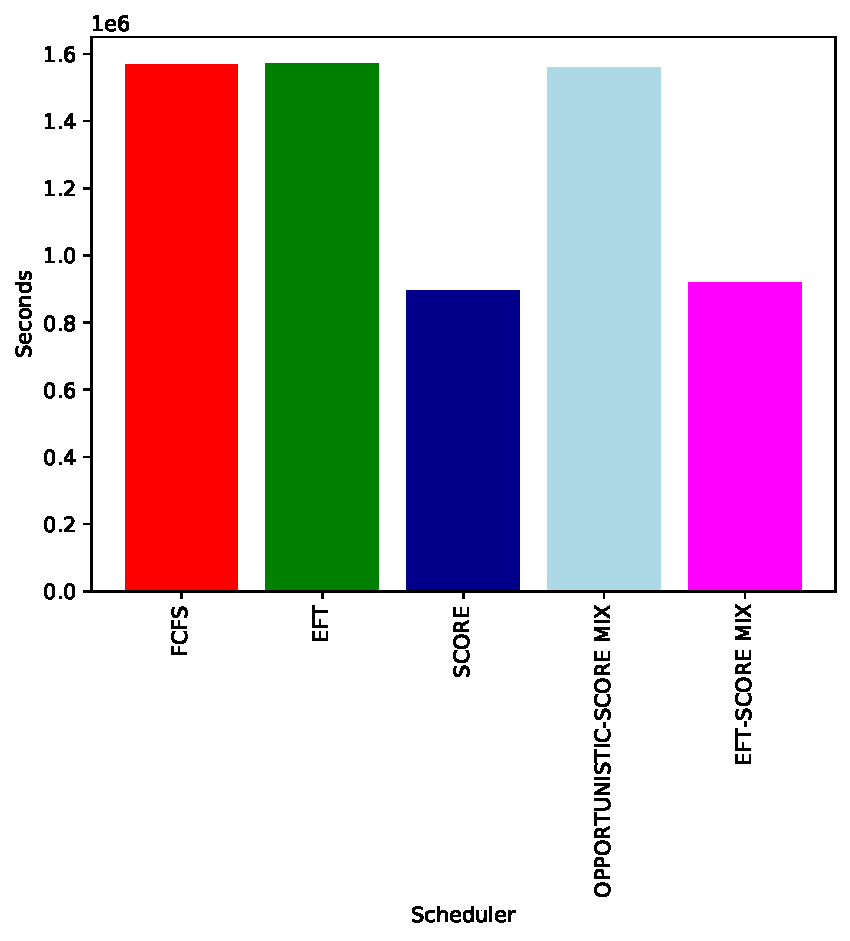
\includegraphics[width=1\linewidth]{../MBSS/plot/Results_FCFS_Score_Backfill_2022-09-09->2022-09-09_V10000_Total_waiting_for_a_load_time_and_transfer_time_450_128_32_256_4_1024.pdf}\caption{Amount of time spent waiting for a file to be available on September 09.}
%~ \label{load.09-09}\end{figure}

Despite greatly reducing the amount of file transfers as can be seen on Figure~\ref{stretch.09-09}b, LEA and LEM
do not manage to beat FCFS in terms of stretch (see Figure~\ref{stretch.09-09}a). 
LEO however has a smaller stretch than FCFS. 
LEA suffers from the same issues as on the last workload: the cluster is
not completely fully used, so 
the locality prevents us from using all the available cores.
However, why does LEM have similar results?

\subsubsection{A pathological scenario of LEM}

\begin{figure}[t]\centering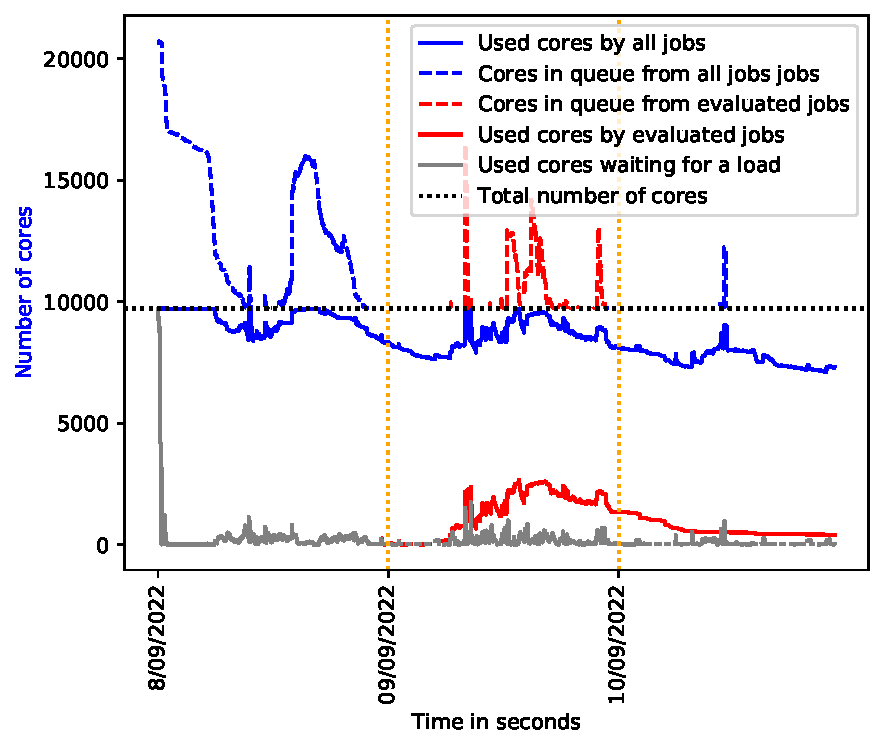
\includegraphics[width=1\linewidth]{../MBSS/plot/Cluster_usage/2022-09-09->2022-09-09_V10000_Fcfs_Used_nodes_Reduced_450_128_32_256_4_1024_core_by_core.pdf}\caption{Visualization of the utilization rate of the cluster on the workload of September 9 with FCFS.}\label{cluster_09-09_fcfs}\end{figure}
\begin{figure}[t]\centering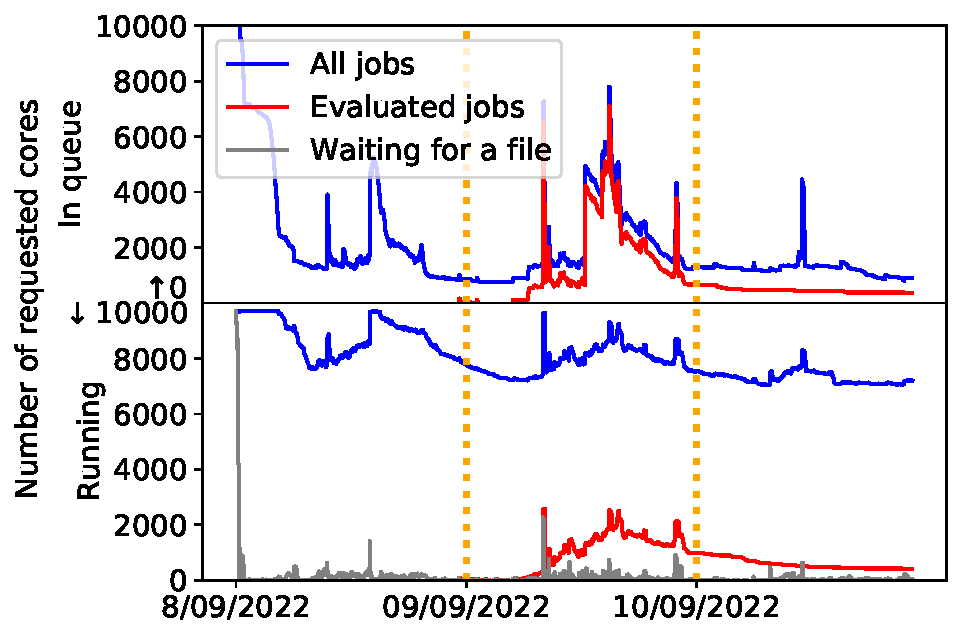
\includegraphics[width=1\linewidth]{../MBSS/plot/Cluster_usage/2022-09-09->2022-09-09_V10000_Fcfs_with_a_score_mixed_strategy_x500_x1_x0_x0_Used_nodes_Reduced_450_128_32_256_4_1024_core_by_core.pdf}\caption{Visualization of the utilization rate of the cluster on the workload of September 9 with LEM.}\label{cluster_09-09_lem}
\end{figure}

The workload of September 9, managed by FCFS (see Figure~\ref{cluster_09-09_fcfs})
results in a cluster that alternates between full utilization and an approximately 80\% utilization rate.
Thus the queue of requested cores alternates between a few thousands and 0.

Figure~\ref{cluster_09-09_lem} represents the same experiment with LEM.
We can see that the queue of requested cores never hits 0.
In this case, the occupation rate is just above 80\%, but not fully
100\%\todo[inline]{Sam: "then why did you choose 80\%? What would choosing
100\% have gotten?". Max: Okay I answered in the next 3 sentences. Is it alright?}, thus LEM stays on the same strategy as LEA.
The threshold to switch between EFT and LEA is set to 80\%. 
This value was found experimentally by testing different thresholds on various types of workloads (see the different cluster's usage in Sections~\ref{sec.07-16}, \ref{sec.09-09}, \ref{sec.03-26} and \ref{sec.08-16}).
This threshold can vary depending on the cluster and it's different utilizations scenarios, and can be found following the same methodology.
Following LEA's strategy is a sub-optimal heuristic when the cluster is not fully saturated.
It creates a queue of jobs that, as long as the cluster's utilization is above 80\%, won't
be scheduled on a node for a long time unless it can re-use their file.
Normally, with this behavior, using LEA leaves a lot of unused nodes that allows LEM
to periodically switch to EFT. But in the case of an almost 
saturated cluster, we still stay above 80\% while not completely using the cluster,
resulting in this queue of jobs clearly visible on the top half of Figure~\ref{cluster_09-09_lem}.
For the jobs in the queue, the stretch is higher than with FCFS, explaining the poor performance of
LEM on Figure~\ref{stretch.09-09}a.

\subsection{A saturated cluster, the great benefits of LEA and LEM}\label{sec.03-26}

\begin{figure}[t]\centering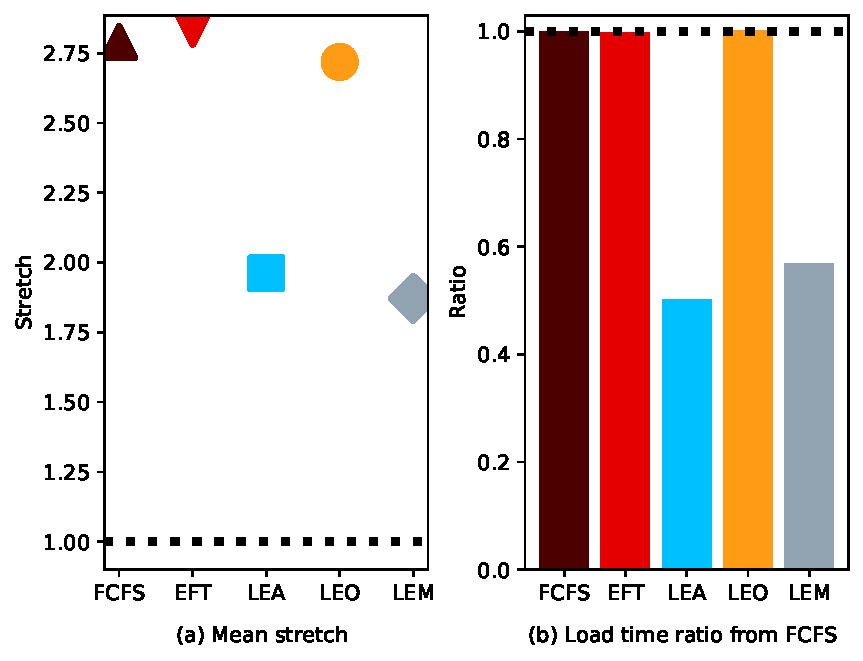
\includegraphics[width=1\linewidth]{../MBSS/plot/Results_FCFS_Score_Backfill_2022-03-26->2022-03-26_V10000_Mean_Stretch_Total_waiting_for_a_load_time_and_transfer_time_450_128_32_256_4_1024.pdf}\caption{Average stretch of all jobs evaluated and total load time on March 26.}
%~ \begin{figure}[t]\centering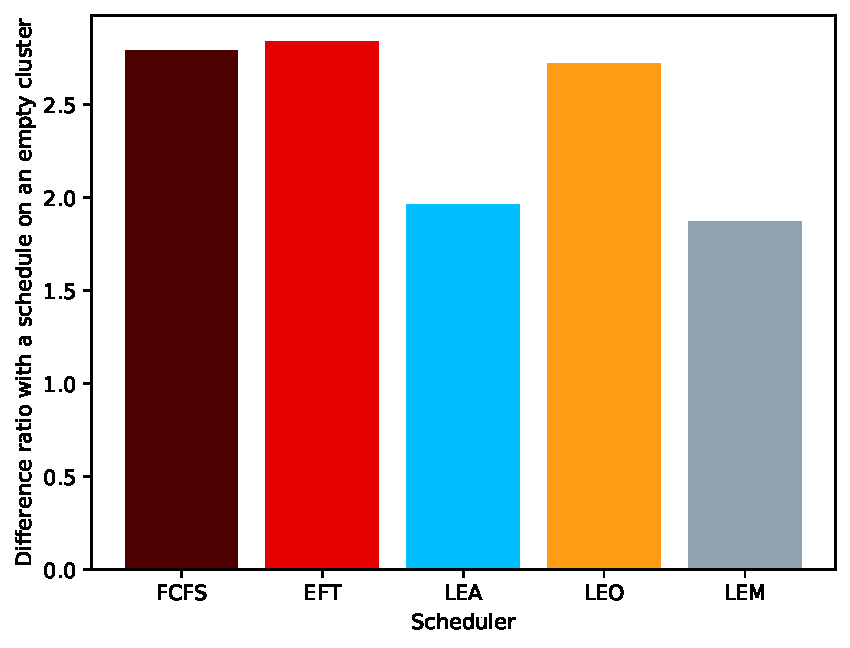
\includegraphics[width=1\linewidth]{../MBSS/plot/Results_FCFS_Score_Backfill_2022-03-26->2022-03-26_V10000_Mean_Stretch_450_128_32_256_4_1024.pdf}\caption{Average stretch of all jobs evaluated on March 26.}
\label{stretch.03-26}\end{figure}
\begin{figure}[t]\centering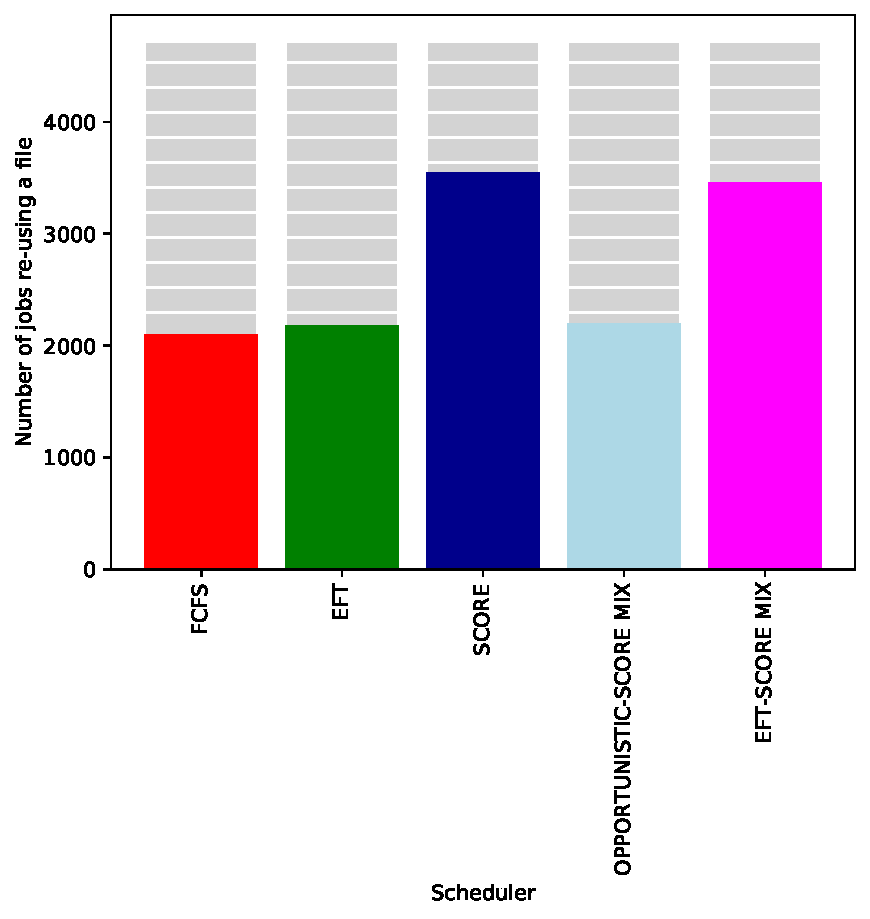
\includegraphics[width=1\linewidth]{../MBSS/plot/Results_FCFS_Score_Backfill_2022-03-26->2022-03-26_V10000_Number_of_data_reuse_450_128_32_256_4_1024.pdf}\caption{Number of evaluated jobs re-using a data on March 26.}\label{reuse.03-26}\end{figure}
\begin{figure}[t]\centering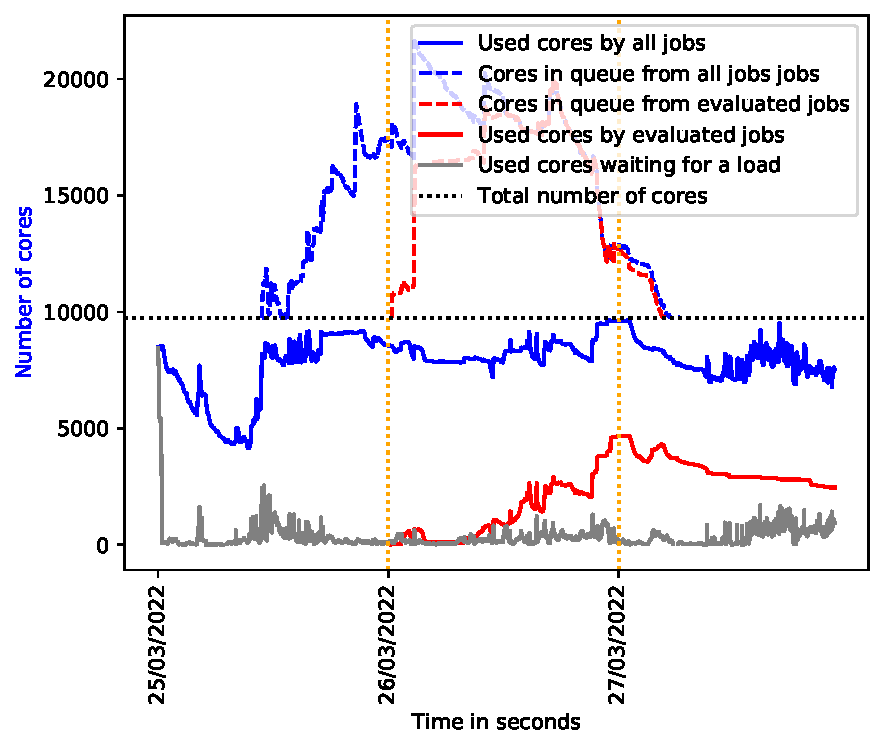
\includegraphics[width=1\linewidth]{../MBSS/plot/Cluster_usage/2022-03-26->2022-03-26_V10000_Fcfs_Used_nodes_Reduced_450_128_32_256_4_1024_core_by_core.pdf}\caption{Visualization of the utilization rate of the cluster on the workload of March 26 with FCFS.}
\label{cluster_usage.03-26_fcfs}\end{figure}
\begin{figure}[t]\centering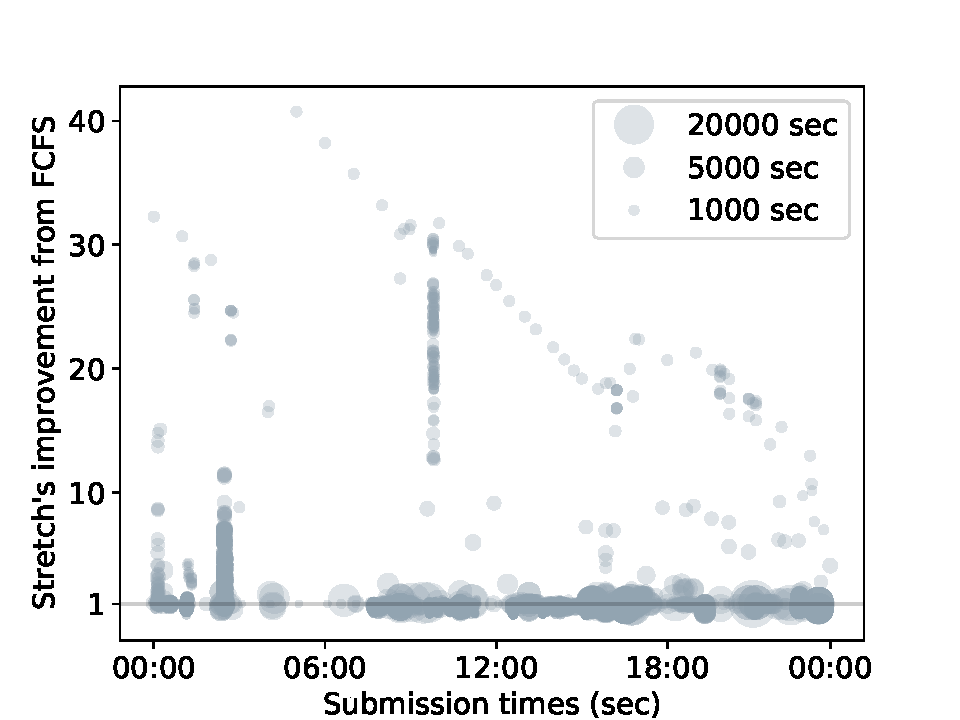
\includegraphics[width=1\linewidth]{../MBSS/plot/Stretch_times/Stretch_times_FCFS_LEM_2022-03-26->2022-03-26_V10000_450_128_32_256_4_1024.pdf}\caption{Stretch times of each job of LEM compared to FCFS on the workload of March 26.}
\label{vs_fcfs_lem_03-26}\end{figure}

The workload presented here saturates the cluster with FCFS. 
Indeed, as we can see on Figure~\ref{cluster_usage.03-26_fcfs}, there is
a queue of several thousands requested cores
for the whole duration of the evaluated day.
In this situation, re-using files has a significant impact
on the queue times. This is confirmed by Figure~\ref{stretch.03-26}:
more data re-use is associated with a smaller stretch for LEA and LEM.
The load time reduction is clearly associated with the number of jobs re-using a file
as observed on Figure~\ref{reuse.03-26}.
On a saturated cluster, filling all the cores with the first jobs of the queue, like FCFS does, is not crucial.
It is more beneficial to group jobs using the same file.
The first few jobs have a longer queue than with FCFS,
but, over time, re-using files causes a snowball effect that reduces the 
queue times of all subsequent jobs.
Moreover, the queue contains enough jobs to fill all the nodes even when grouping them by input file.
We thus avoid the pathological cases presented in sections~\ref{sec.07-16} and \ref{sec.09-09}.
In this case, LEA's strategy, also found in LEM, allows to greatly reduce the mean stretch.
We can observe this, job by job, on Figure~\ref{vs_fcfs_lem_03-26}: very few jobs 
have a speed-up inferior to 1 and a large amount of jobs are above 2. 
% The columns of circles are set of jobs using the same file, that all saved time on the loading phase. 

\subsection{A cluster saturated with small jobs, the best case scenario for LEA and LEM}\label{sec.08-16}

\begin{figure}[t]\centering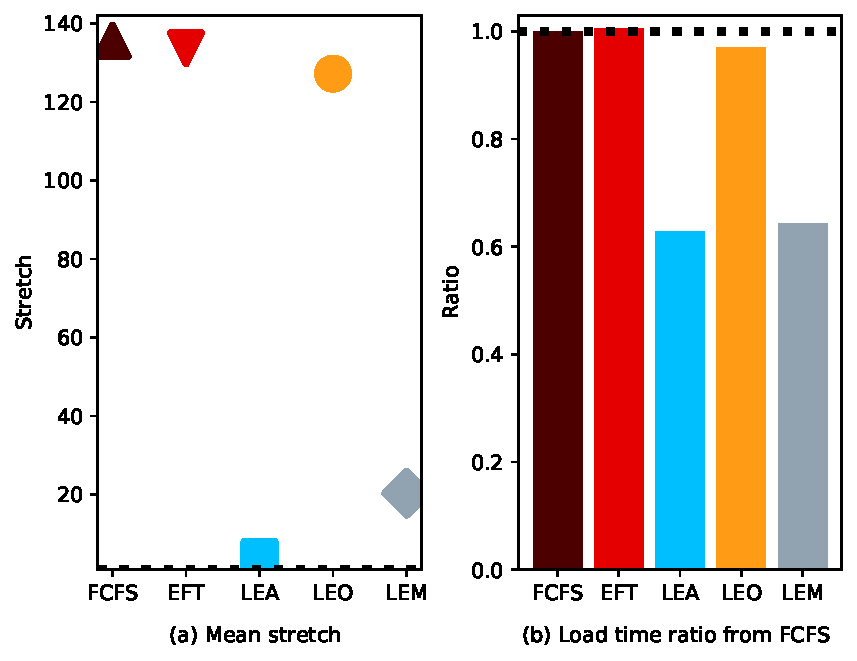
\includegraphics[width=1\linewidth]{../MBSS/plot/Results_FCFS_Score_Backfill_2022-08-16->2022-08-16_V10000_Mean_Stretch_Total_waiting_for_a_load_time_and_transfer_time_450_128_32_256_4_1024.pdf}\caption{Average stretch of all jobs evaluated and total load time on August 16.}\label{stretch.08-16}\end{figure}
%~ \begin{figure}[t]\centering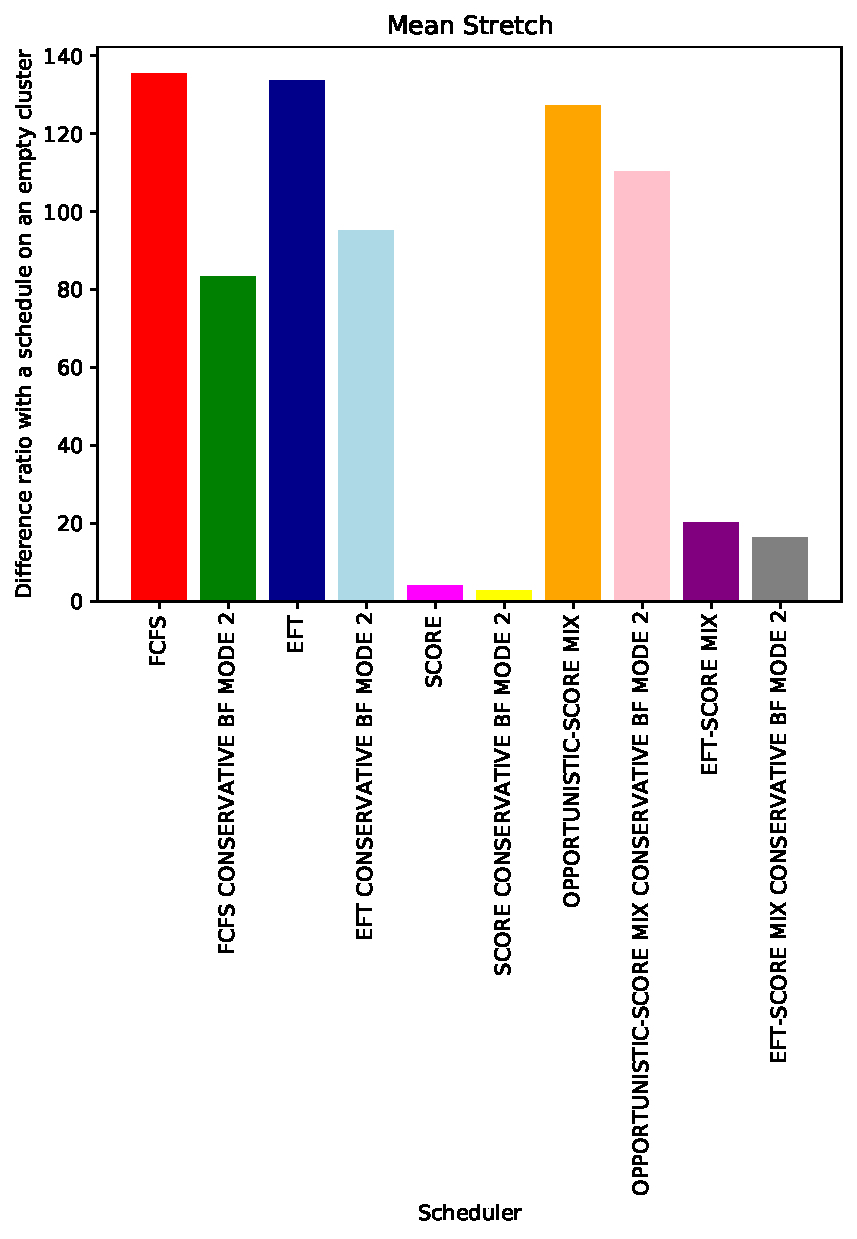
\includegraphics[width=1\linewidth]{../MBSS/plot/Results_FCFS_Score_Backfill_2022-08-16->2022-08-16_V10000_Mean_Stretch_450_128_32_256_4_1024.pdf}\caption{Average stretch of all jobs evaluated on August 16.}\label{stretch.08-16}\end{figure}
\begin{figure}[t]\centering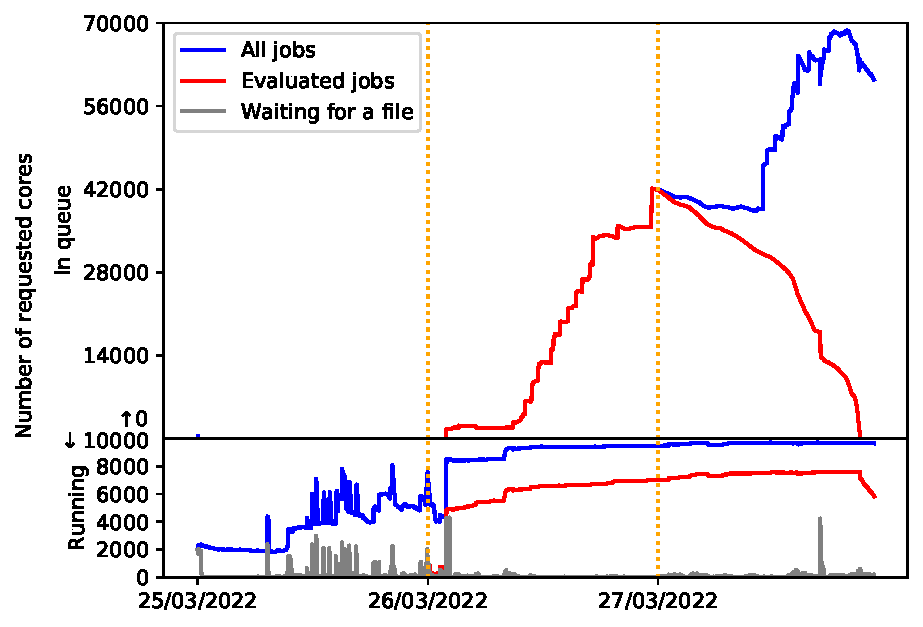
\includegraphics[width=1\linewidth]{../MBSS/plot/Cluster_usage/2022-08-16->2022-08-16_V10000_Fcfs_Used_nodes_Reduced_450_128_32_256_4_1024_core_by_core.pdf}\caption{Visualization of the utilization rate of the cluster on the workload of August 16 with FCFS.}
\label{cluster_usage.08-16_fcfs}\end{figure}
\begin{figure}[t]\centering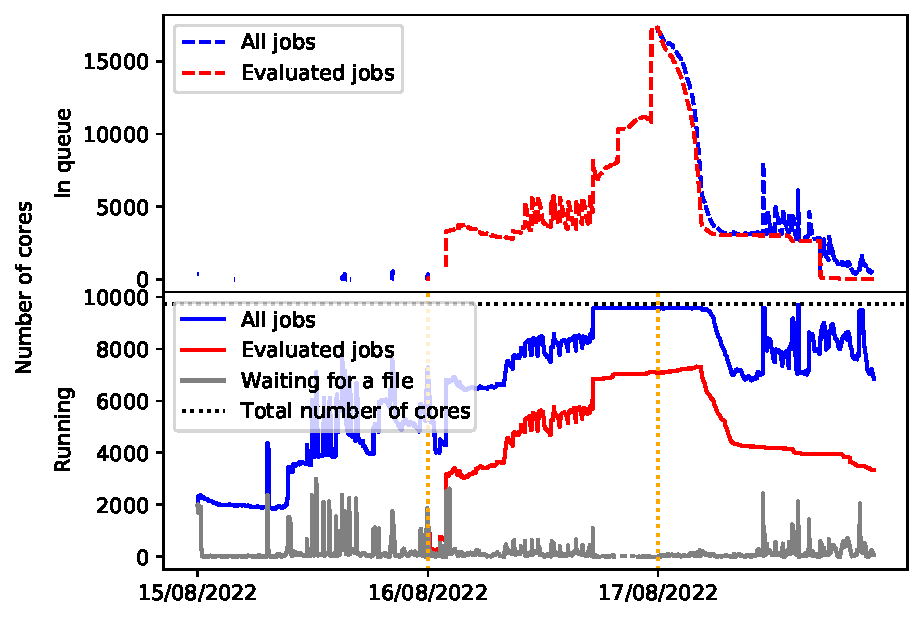
\includegraphics[width=1\linewidth]{../MBSS/plot/Cluster_usage/2022-08-16->2022-08-16_V10000_Fcfs_with_a_score_mixed_strategy_x500_x1_x0_x0_Used_nodes_Reduced_450_128_32_256_4_1024_core_by_core.pdf}\caption{Visualization of the utilization rate of the cluster on the workload of August 16 with LEM.\todo[inline]{Max: I think this figure can be removed, I don't really use it in the explanations.}}
\label{cluster_usage.08-16_lem}\end{figure}

From Figure~\ref{stretch.08-16}a, we observe that LEA has a stretch 33 times smaller than
its competitors. LEM is about 7 times smaller. This drastic diminution is explained
by the two particularities of this workload.
Firstly, it is a workload that heavily saturates the cluster as you can see\todo[inline]{Max: Can we say "as you can see" in an article? Talking directly to the reader.} in Figure~\ref{cluster_usage.08-16_fcfs}
(note that the Y axis of the top half is modified here to denote the large amount of requested cores compared to the total amount of cores).
So, for the same reasons as in Section~\ref{sec.03-26}, LEA and LEM largely reduce load times.
Secondly, it is a workload largely composed of jobs that are short and using less than five cores.
%The size of a file is always between 6.4 and 128GB.
On shorter jobs, the proportion of the duration spent on the file transfer is very high. 
Thus, reducing the transfer time of small jobs has a much greater effect on the stretch, resulting in this 
drastic reduction for LEA and LEM, as can be seen on Figure~\ref{cluster_usage.08-16_lem}.

\subsection{Aggregated results on 44 different evaluated workloads}

\begin{figure}[t]\centering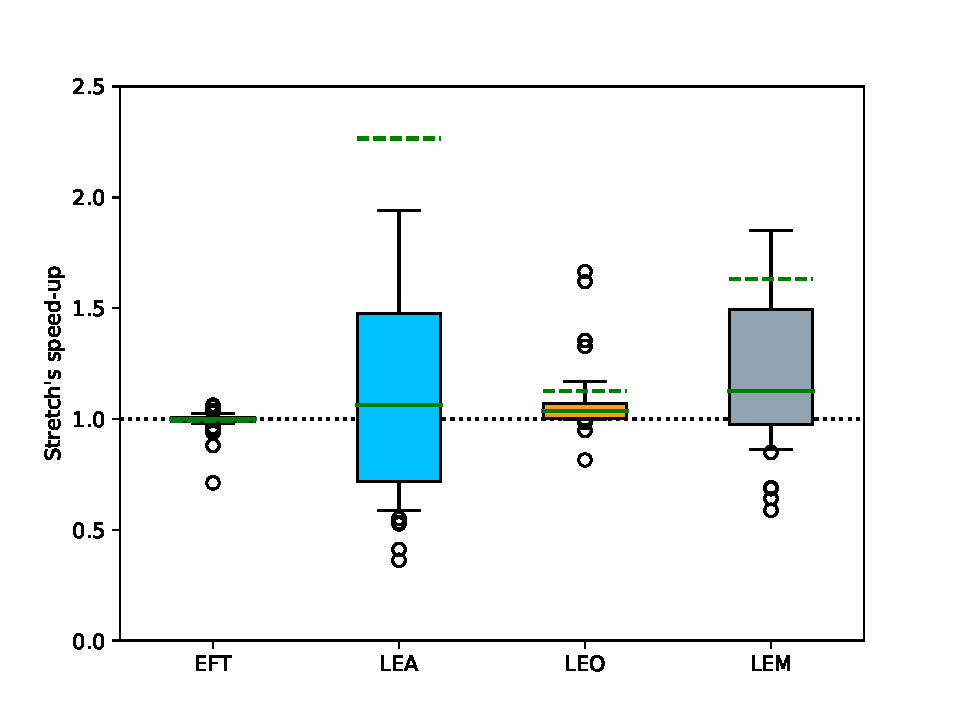
\includegraphics[width=1\linewidth]{../MBSS/plot/Boxplot/box_plot_mean_stretch_all_workloads.pdf}\caption{Mean stretch's improvement from FCFS on all evaluated workloads. The whiskers are the octiles. The solid green line represent the median and the dashed one the mean.}\label{boxplot.all}\end{figure}
\begin{figure}[t]\centering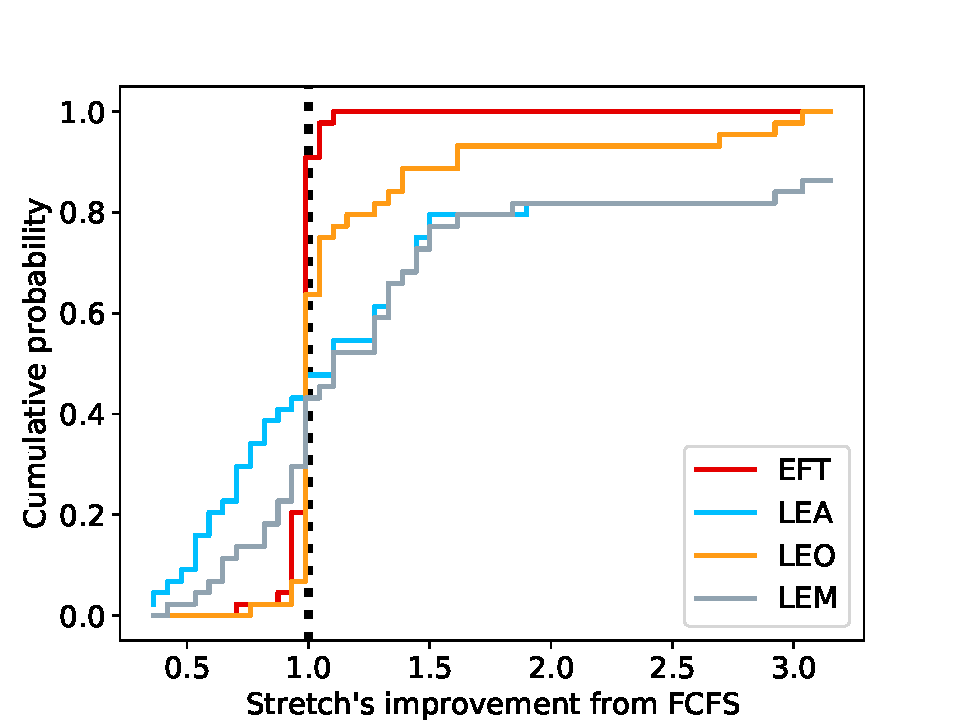
\includegraphics[width=1\linewidth]{../MBSS/plot/ECDF/ecdf_mean_stretch_all_workloads.pdf}\caption{Empirical distribution function of the mean stretch's improvement from FCFS on all evaluated workloads.}\label{ecdf}\end{figure}
\begin{figure}[t]\centering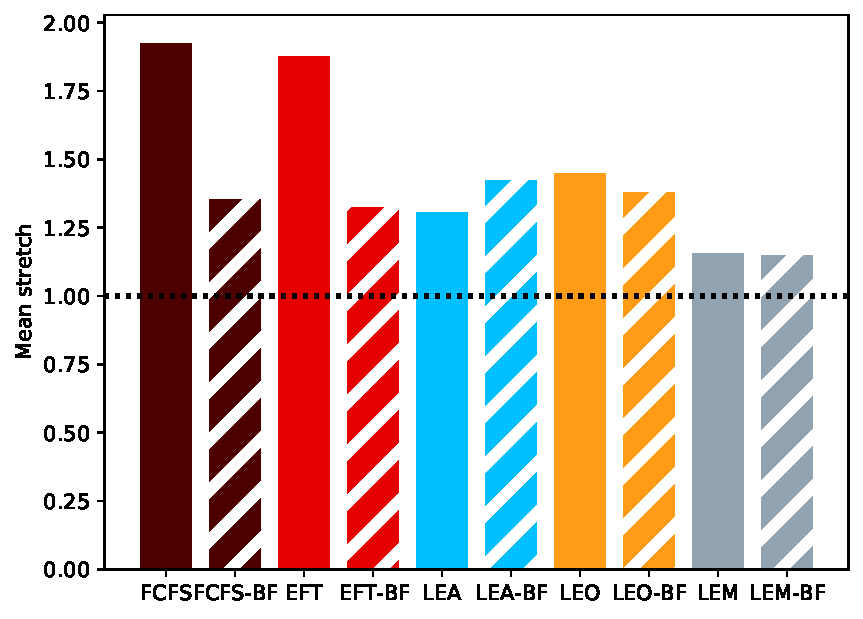
\includegraphics[width=1\linewidth]{../MBSS/plot/BF_AND_NON_BF_Results_FCFS_Score_Backfill_2022-01-28->2022-01-28_V10000_Mean_Stretch_450_128_32_256_4_1024.pdf}\caption{Average stretch of all jobs evaluated on January 28 with and without backfilling.\todo[inline]{Max: Do you want to keep this or I put the old one with bars and hashed bars for backfilling?}}\label{stretch.01-28}\end{figure}
\begin{figure}[t]\centering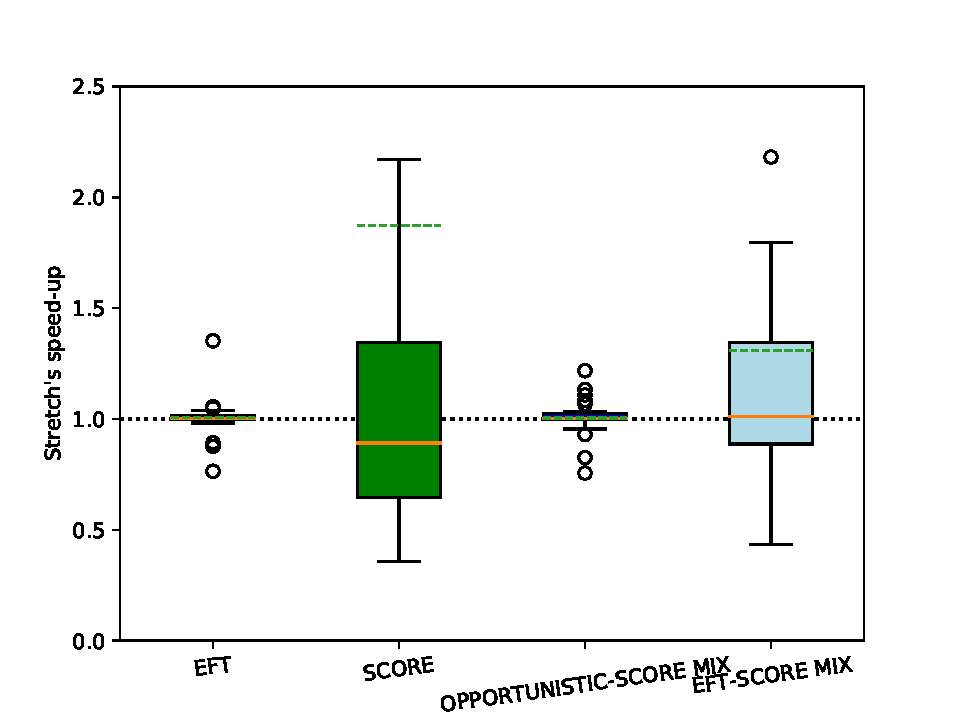
\includegraphics[width=1\linewidth]{../MBSS/plot/Boxplot/box_plot_mean_stretch_all_workloads_bf.pdf}\caption{Mean stretch's improvement from FCFS-BF on all evaluated workloads.}\label{boxplot.all_bf}\end{figure}

We evaluated our 5 schedulers on 44 different days.
Figure~\ref{boxplot.all} represents boxplots from the aggregated
results of the stretch's improvement compared to FCFS on these evaluations.
On this figure, 50\% of the results are within the box.
The whiskers delimit the octiles, thus 75\% of the results are contained
within the whiskers. This also means that between the lower side of the box and the maximum value,
we find 75\% of the results (and similarly between the upper side of the box and the minimum value).
The solid green lines show the median while the dashed ones show the mean stretch's improvement compared to FCFS. 
Each white circle is an outlier whose improvement is in the first or last octile.
A result above the black dotted line is an improvement compared to FCFS' mean stretch.

As in the previous results, we observe that EFT does not bring any real improvement compared to FCFS.
For LEA, LEO and LEM, the medians are respectively 1.12, 1.03 and 1.13. 
However the mean values are much higher at 2.26, 1.21 and 1.76.

We can explain the larger mean values for LEA and LEM from the good performance of LEA's strategy
on heavily saturated clusters (see Section~\ref{sec.03-26} and \ref{sec.08-16}).
In these cases, the mean stretch values of LEA or LEM are much smaller than those of FCFS or EFT.
Re-using the same files is not detrimental to the filling of all the nodes because there are 
enough jobs to cover all nodes.
A large decrease in the time spent waiting for a file greatly reduces the stretch of each job.
Compared to LEA, LEM has a smaller mean value.
However 75\% of its results are above 1, i.e. an improvement, whereas for LEA, only approximately 57\% of the results are above 1. 
LEM is a more versatile strategy and offers higher sustained performance on non-saturated cluster at the cost
of fewer extreme improvements on heavily saturated clusters.
The maximum values are not shown. For LEA and LEM, 6 outliers are above the upper whisker with 
a maximum respectively at 33.5 and 6.7.

From the same data shown on Figure~\ref{boxplot.all}, we plot an empirical distribution function on Figure~\ref{ecdf}.
EFT's low variance is clearly visible in the sudden jump in probability around an improvement of 1.
It is interesting to note that for LEA and LEM, 20\% of the results are above an improvement of 300\%.
In addition, thanks to its switch between the strategies of EFT and LEA, LEM clearly reduces
performance losses on the left of the black line.
We can also learn from this figure that LEO is in every respect a better version of EFT.
At no point, it shows a higher cumulative probability before 1. Above 1 it shows significantly better
results beyond an improvement of 20\%.

Thus, without backfilling, LEM is the best strategy to observe significant improvements.
It can compute jobs between 1 and 1.5 times faster in 50\% of the cases,
between 1.5 and 3 times faster in 12.5\% of the cases and between 3 and 6.7 times faster in 12.5\% of the cases.
It is slower in only 25\% of the workloads, and 12.5\% of those are within a 0.15 slow-down.
LEO is a more sustained strategy with 87.5\% of its results above an improvement of 1, which shows that our opportunistic
strategy is much more consistent, while still having great improvements in some cases, as can be seen with the outliers above the 1.5 mark.

\todo[inline]{Max: Below, when discussing backfilling, should I call everyone with a -BF or it's not necessary?}
Figure~\ref{boxplot.all_bf} shows the results with the backfilling version of our
schedulers and compared to FCFS with backfilling (FCFS-BF) on all workloads.
We can notice that with backfilling, our schedulers have smaller improvements.
To understand this we can look at Figure~\ref{stretch.01-28}. We can see that 
with backfilling 
% (hashed bars),
(hollow markers),
the mean stretch is much lower for FCFS-BF and EFT-BF. 
However, our strategies do not benefit from backfilling as much as FCFS-BF does for two reasons:
\begin{itemize}
	\item Even if we consider data locality when backfilling, trying to fill a node as much as possible and optimizing data re-use are two contrary goals. 
	Backfilling a job can compromise a re-use pattern that was planned by our locality-aware strategy, thus reducing the total 
	amount of re-used files.
	\item Our strategies are already able to nicely fill the nodes without needing backfilling.
	Grouping jobs by input file implies that similar jobs end up on the same nodes.
	Jobs having the same duration and number of requested cores can much more easily fill a node to its fullest than a completely heterogeneous set of jobs.
	Consequently, the shortfall without backfilling is much lower for LEA-BF, LEO-BF and LEM-BF, than for FCFS-BF and EFT-BF.
\end{itemize}
Thus, compared to FCFS-BF, we still reduce the total queue time with backfilling.
However, the difference is less significant. One can observe an example of this
in Figure~\ref{stretch.01-28} by looking at LEM and LEM-BF compared to FCFS and FCFS-BF.

In Figure~\ref{boxplot.all_bf}, for both EFT-BF and LEO-BF, the improvements are not significant.
LEA-BF has a median slightly worse than our competitor. However it still
achieves a better mean.

Out of our four heuristics, LEM-BF is the best compromise.
It is better than FCFS-BF in more than 50\% of the cases, 
with 25\% of those results above an improvement of 1.35.
Moreover, improvements are still important on heavily saturated clusters, as can be seen with the outliers.
Among the slow-downs, only 25\% are superior to 0.15.

\todo[inline]{LM: should we say somewhere that we tested with stronger data persistence and it did not really helps?}

\section{Conclusion}\label{sec.conclusion}

\todo[inline]{Max: - Results of LEA, LEO and LEM - Fairness - Advance reservation - Tune LEM - Improve locality of LEO - Tune BF for LEA, LEO and LEM - Talk about the genericity of our problem?}

\bibliographystyle{IEEEtran}
\bibliography{ref.bib}
\end{document}
